\chapter{Diseño y Desarrollo}
\label{cap:diseno-desarrollo}

\newcommand{\partesep}[1]{%
  \bigskip
  \begin{center}\hrulefill\quad\textbf{\large #1}\quad\hrulefill\end{center}
  \addcontentsline{toc}{section}{#1}%
  \nopagebreak\medskip}

\section{Introducción del capítulo}

El capítulo~\ref{cap:analisis} establece \emph{qué} debe hacer el sistema, y este capítulo explica \emph{cómo} se ha construido, en dos partes diferenciadas.

La primera, diseño, parte de que el usuario principal es una persona mayor con posible deterioro visual y brecha digital. Esta primera parte recoge las reglas de diseño, las decisiones de accesibilidad, con los criterios WCAG~2.2 que las respaldan y el contraste calculado sobre la paleta, y el paso de los bocetos al código.

La segunda, desarrollo, describe el sistema construido: el \emph{stack}, la arquitectura y el papel del servidor, la seguridad, la voz, el ciclo de vida de una conversación con su análisis y su memoria, el consentimiento informado conforme al RGPD y la conversación por escrito. Cada decisión técnica se justifica donde se describe. El capítulo cierra con la cronología del desarrollo.

\partesep{Parte I: Diseño}

\section{Principios de diseño}

\subsection{Diseño centrado en la persona mayor}

El problema que aborda el sistema, la soledad no deseada en personas mayores (capítulo~\ref{cap:marco-teorico}), determina un usuario con un perfil muy concreto: edad avanzada, agudeza visual y sensibilidad al contraste reducidas, y una relación con la tecnología que a menudo es de desconfianza más que de desconocimiento. Para ese usuario, los principios del capítulo~\ref{cap:introduccion} se concretan en tres reglas que actúan como restricciones de diseño y no como recomendaciones.

\textbf{La voz es la interfaz primaria; la pantalla es su respaldo.} La conversación hablada es la modalidad de interacción que menos alfabetización digital exige y la única que no se degrada con la pérdida de agudeza visual. Por eso la pantalla principal del mayor tiene un solo control grande, el botón de micrófono; lo demás es información y accesos secundarios: una fila inferior con emergencia, teclado y Ajustes, y <<Mi semana>> cuando hay algo que enseñar. El texto de la respuesta se muestra a la vez que se pronuncia porque la redundancia sensorial beneficia también a quien oye mal, no porque se espere que el usuario lea.

\textbf{La previsibilidad prima sobre la inteligencia.} La aplicación nunca cambia por su cuenta cómo se ve ni cómo habla. El tamaño de la letra, el volumen, la velocidad de la voz y el tiempo que espera al mayor solo cambian cuando lo decide él o su familiar, aunque habría sido sencillo que el asistente los ajustara solo: le bastaría una función más, como la que usa para guardar el nombre del mayor, para subir el volumen cuando este pide a menudo que le repitan algo. No se hace porque un cambio que nadie ha pedido desorienta a quien ya maneja el teléfono con inseguridad; el mayor no sabría por qué la aplicación ha cambiado; y una deducción equivocada le haría perder la confianza en ella, que tanto cuesta ganar.

\textbf{Ningún camino puede terminar en un callejón sin salida.} Los errores se comunican con texto persistente en pantalla, no con avisos efímeros: un \code{SnackBar} (widget flotante de Flutter) que se desvanece en cuatro segundos es inservible para quien tarda más de cuatro segundos en leerlo.

\subsection{Revelación progresiva}

La revelación progresiva aplica al diseño el tercer principio del capítulo~\ref{cap:introduccion}, el cuidado compartido. El sistema atiende a dos perfiles de mayor, Independiente y Vinculado, que difieren en quién gestiona la configuración y no en qué hacen con la aplicación. Construir dos flujos, o dos aplicaciones, duplicaría las pantallas que mantener, algo inviable para un desarrollador único, y las dos versiones acabarían divergiendo.

Por eso hay un único núcleo de aplicación, la pantalla de chat por voz, que sirve a los dos perfiles. La diferencia se resuelve \emph{mostrando u ocultando} capacidades según el atributo \code{autonomy} del modelo de usuario. La autonomía es un dato de configuración, no una identidad distinta, en coherencia con el modelo conceptual de dominio del capítulo~\ref{cap:analisis}.

En el código, el botón de Ajustes de la pantalla principal se muestra si la función pura\footnote{Una función pura es aquella cuyo resultado depende solo de los argumentos que recibe, sin leer ni modificar nada fuera de ella: con los mismos argumentos devuelve siempre lo mismo, y puede probarse sin base de datos ni interfaz.} \code{visibleSettingsRows(user)} devuelve alguna fila de ajustes visible para ese usuario. La pantalla de ajustes se construye sobre la misma lista y con la misma regla de visibilidad por fila. Si el botón y la pantalla calculasen su visibilidad por separado, acabarían divergiendo, y el resultado sería un botón que abre una pantalla vacía, un fallo tan grave para este usuario como un botón que no responde.

El enumerado \code{AutonomyStatus} añade a los dos perfiles de RF-1 dos valores técnicos: \code{linked}, que describe al familiar ya emparejado, y \code{none}, el estado previo a elegir modo.

\section{Accesibilidad}
\label{sec:accesibilidad}

\subsection{Cumplimiento WCAG 2.2 AA: objetivos y alcance}

RNF-1 fija como objetivo el nivel~AA de las \emph{Web Content Accessibility Guidelines}~2.2 \autocite{wcag}. La norma está redactada para contenido web, pero sus criterios de éxito de perceptibilidad y operabilidad son independientes del medio y se aplican aquí a una interfaz nativa Flutter sin pérdida de sentido.

El objetivo AA se aplica a la interfaz del mayor, no al panel del familiar. El familiar es un adulto al que no se le suponen limitaciones, que maneja un panel de gestión convencional, y el mayor es el usuario cuyas limitaciones definieron el proyecto. En el código, esa diferencia se traduce en dos temas separados, \code{elderTheme} y \code{companionTheme}, con reglas tipográficas y de tamaño distintas.

Los colores y los tamaños mínimos de la letra y de los elementos táctiles viven en una única clase, \code{AppTheme} (\code{lib/core/theme/app\_theme.dart}), y no en cada pantalla. Cualquier pantalla del mayor hereda las propiedades de accesibilidad de entrada.

\subsection{Decisiones de interacción}

RNF-2 y RNF-4 concretan la operabilidad en dos reglas que se han aplicado sin excepción.

\textbf{Superficies táctiles de al menos $80\times80$ píxeles lógicos.} Los botones de ancho completo del mayor y las filas de la lista de ajustes miden 88~px de alto (\code{emergencyButtonMinHeight}), el doble de los $44\times44$~px CSS del criterio 2.5.5 (\emph{Target Size (Enhanced)}) de WCAG~2.2, el más exigente de la norma. Los botones de icono de la pantalla principal y el de <<Enviar>> se quedan en el mínimo del requisito, $80\times80$. El botón de micrófono, control primario de la aplicación, mide 200~px de diámetro en teléfono y 260~px en tableta, y mengua cuando la letra pasa de <<Normal>>, hasta el 70~\% con <<La más grande>>: quien amplía la letra necesita sitio para leer la respuesta más que un botón aún mayor, y con 140~px sigue siendo el control más grande de la pantalla.

\textbf{Solo pulsación simple.} Toda la interacción del mayor se resuelve con \code{onTap}: no hay \code{onLongPress}, ni \code{onDoubleTap}, ni acciones que se ejecuten deslizando. El temblor y la pérdida de destreza fina hacen que el doble toque y la pulsación mantenida fallen con frecuencia. Nielsen Norman Group documenta este patrón de dificultad en usuarios mayores \autocite{Kane2019}. Cuando la letra ampliada no cabe en la pantalla, el contenido se desplaza, título incluido, porque el título va en el propio contenido y no en la barra superior, que lo cortaría; cada acción sigue siendo un botón visible. Como cada acción necesita su propio control visible, las pantallas tienen pocas acciones, y eso también las simplifica.

La pantalla de emergencia se presenta como ruta a pantalla completa (\code{fullscreenDialog}) y no como diálogo modal, porque la barrera de un diálogo, la zona que lo cierra al tocarla, es un sitio más donde equivocarse en mitad de una emergencia. Por el mismo motivo, la aplicación abre el marcador del sistema con el número ya escrito, mediante un URI \code{tel:}. Marcar directamente habría exigido el permiso peligroso \code{CALL\_PHONE} y abierto la puerta a una llamada accidental al 112; el coste es un toque más, justo donde una equivocación es más cara.

Las pantallas de consentimiento, <<Mi semana>> y el modo teclado comparten un botón común del mayor, \code{ElderButton}, que fija el ancho completo, los 88~px de alto y el escalado del texto. Por estas reglas, el consentimiento se recoge con dos botones grandes y no con una casilla, cuyo tamaño habitual incumpliría RNF-2, y <<Mi semana>> cuenta la semana con frases y no con gráficas. Ambos se desarrollan en los apartados~\ref{sec:privacidad} y~\ref{sec:bienestar}.

\subsection{Tipografía y escalado dinámico}

RNF-3 fija cuerpo $\geq 20$~sp y títulos $\geq 28$~sp. El sistema de diseño define cuatro tamaños, \code{fontButton} (20), \code{fontMedium} (24), \code{fontLarge} (32) y \code{fontHuge} (40), y no existe ningún tamaño por debajo de 20 en las pantallas del mayor.

Sobre ese mínimo actúa el multiplicador \code{textSizeMultiplier} de \code{UserPreferences}, cuyo valor por defecto es 1.2 y no 1.0. El valor de fábrica ya está sesgado hacia la accesibilidad, para que en el caso más probable (un mayor que nunca toque la configuración) se reciba una tipografía ampliada por omisión. El mismo criterio se aplica a \code{speechRate}, cuyo valor por defecto (0.4 en la escala de \code{flutter\_tts}) produce una voz deliberadamente más lenta.

El propio mayor puede ajustar desde Ajustes cuatro escalas: el tamaño de la letra, el volumen y la velocidad de la voz, y el tiempo que la aplicación le espera en silencio antes de responder; elige además la voz que le habla (apartado~\ref{sec:voz}). El menú se agrupa por lo que el mayor quiere cambiar, en cuatro entradas a lo sumo (<<Mis datos>>, con el contacto de emergencia y la cuenta; el tamaño de la letra; <<Cómo hablamos>>, y <<Mis conversaciones>>), para que quepa entero en una pantalla sin desplazarse. Las escalas se presentan como \textbf{peldaños con nombre} (<<Normal>>, <<Grande>>, <<Muy grande>>\ldots) y no como deslizadores. El panel del familiar, pensado para un adulto con mayor destreza tecnológica, conserva los deslizadores.

El escalado es dinámico y se aplica en tiempo de construcción del widget, multiplicando cada tamaño base por el factor leído del documento de usuario (\code{AppTheme.font* * textScale}). Al ser el documento la fuente reactiva descrita en el apartado~\ref{sec:ssot}, la letra del mayor cambia de tamaño en pantalla en torno a un segundo cuando el familiar mueve el deslizador en su dispositivo, sin reiniciar la aplicación ni intervención alguna del mayor.

\subsection{Teoría del color aplicada a personas mayores}
\label{sec:color}

Dos cambios de la visión con la edad afectan a las decisiones de paleta. El primero es el \textbf{amarilleamiento y aumento de densidad del cristalino}: con la edad, el medio ocular absorbe progresivamente más luz de longitud de onda corta, de modo que llega menos luz azul a la retina. \textcite{Pokorny1987} cuantificaron esta pérdida de transmisión y establecieron el modelo de densidad óptica del cristalino en función de la edad que sigue siendo referencia. Por eso la discriminación del color empeora de forma \textbf{asimétrica}, y los defectos de la población mayor son sobre todo del tipo azul-amarillo.

El segundo fenómeno es la \textbf{pérdida de sensibilidad al contraste}, independiente de la agudeza y más acusada en condiciones de baja luminancia, que \textcite{Owsley2011} revisa como uno de los cambios funcionales mejor documentados del envejecimiento visual. Por ambos motivos, los elementos se distinguen por el contraste de luminancia, medido según WCAG, y nunca por el tono. En particular se evita el texto azul de bajo contraste y las combinaciones azul o violeta sobre fondo oscuro, que son exactamente las que el amarilleamiento del cristalino degrada.

El color primario es Canela (\code{\#A0522D}), elegido entre cuatro tonos cálidos, y el fondo es un blanco cálido (\code{\#FFF8F0}) en lugar de blanco puro. Los tokens de la pantalla de emergencia se eligieron con el contraste calculado por adelantado y anotado en el propio código.

La \autoref{tab:contraste} recoge las razones de contraste de la paleta del mayor, calculadas según la fórmula de luminancia relativa de WCAG~2.2 \autocite{wcag} sobre el fondo \code{\#FFF8F0}.

\begin{table}[htbp]
    \centering
    \caption{Razones de contraste de la paleta del mayor sobre el fondo \texttt{\#FFF8F0}, calculadas según WCAG~2.2. Umbrales: 4{,}5:1 (AA, texto normal), 7:1 (AAA, texto normal), 3:1 (1.4.11, elementos no textuales).}
    \label{tab:contraste}
    \begin{tabularx}{\textwidth}{@{}>{\RaggedRight\arraybackslash}X c c >{\RaggedRight\arraybackslash}X@{}}
        \toprule
        \textbf{Token} & \textbf{Valor} & \textbf{Ratio} & \textbf{Cumple} \\
        \midrule
        \texttt{elderTextPrimary} (cuerpo)    & \#1A1A2E & 16{,}19:1 & AAA \\
        \texttt{elderTextSecondary}            & \#4A4A6A & 8{,}04:1  & AAA \\
        \texttt{emergency112}                  & \#A4031F & 7{,}63:1  & AAA \\
        \texttt{emergencyContactCall}          & \#1B5E20 & 7{,}47:1  & AAA \\
        \texttt{elderPrimary}                  & \#A0522D & 5{,}33:1  & AA (no AAA) \\
        \texttt{elderEmergency}                & \#D90429 & 4{,}98:1  & AA (no AAA) \\
        \texttt{elderTalking} (\emph{Respondiendo}) & \#2D8A4E & 4{,}10:1  & 1.4.11 (no textual) \\
        \texttt{elderThinking} (\emph{Pensando})    & \#C1691B & 3{,}76:1  & 1.4.11 (no textual) \\
        \bottomrule
    \end{tabularx}

\end{table}

Toda la paleta supera el umbral que le corresponde. El texto de cuerpo alcanza 16{,}19:1, muy por encima del AAA, y el camino crítico de emergencia supera 7:1 en los dos botones. Los colores de los estados \emph{Respondiendo} y \emph{Pensando} solo tiñen el anillo y el icono del micrófono, nunca texto, así que se miden con el umbral de 3:1 del criterio 1.4.11 (\emph{Non-text Contrast}), y lo superan también sobre el relleno tenue del propio color que ocupa el interior del botón.

Además, el estado del asistente nunca se comunica solo por el color: hay simultáneamente una etiqueta de texto en tamaño grande (\emph{<<Te escucho\ldots>>}, \emph{<<Pensando\ldots>>}, \emph{<<Respondiendo\ldots>>}), un icono distinto por estado (micrófono, reloj de arena, altavoz) y un cambio de grosor del borde. Esto satisface el criterio 1.4.1 (\emph{Use of Color}), que exige que el color no sea el único medio de transmitir información, y permite usar la interfaz a quien tiene daltonismo o el defecto azul-amarillo descrito arriba.

\section{Evolución del diseño de interfaz: del boceto al código}
\label{sec:evolucion-diseno}

El diseño de interfaz no se abordó directamente en Flutter. Pasó por dos etapas, el boceto a lápiz y el wireframe a escala, antes de programarse.

\subsection{Bocetos a mano}

La primera etapa fueron bocetos a lápiz en libreta. Permitieron enunciar y desechar una distribución de pantalla en menos de un minuto, un coste lo bastante bajo como para explorar alternativas que no se explorarían si cada una costase una hora de código. En esta fase se fijó que la pantalla principal del mayor tuviera un solo control grande y centrado, con todo lo demás como información o accesos secundarios en los márgenes, y ninguna iteración posterior lo cambió.

\begin{figure}[htbp]\centering
  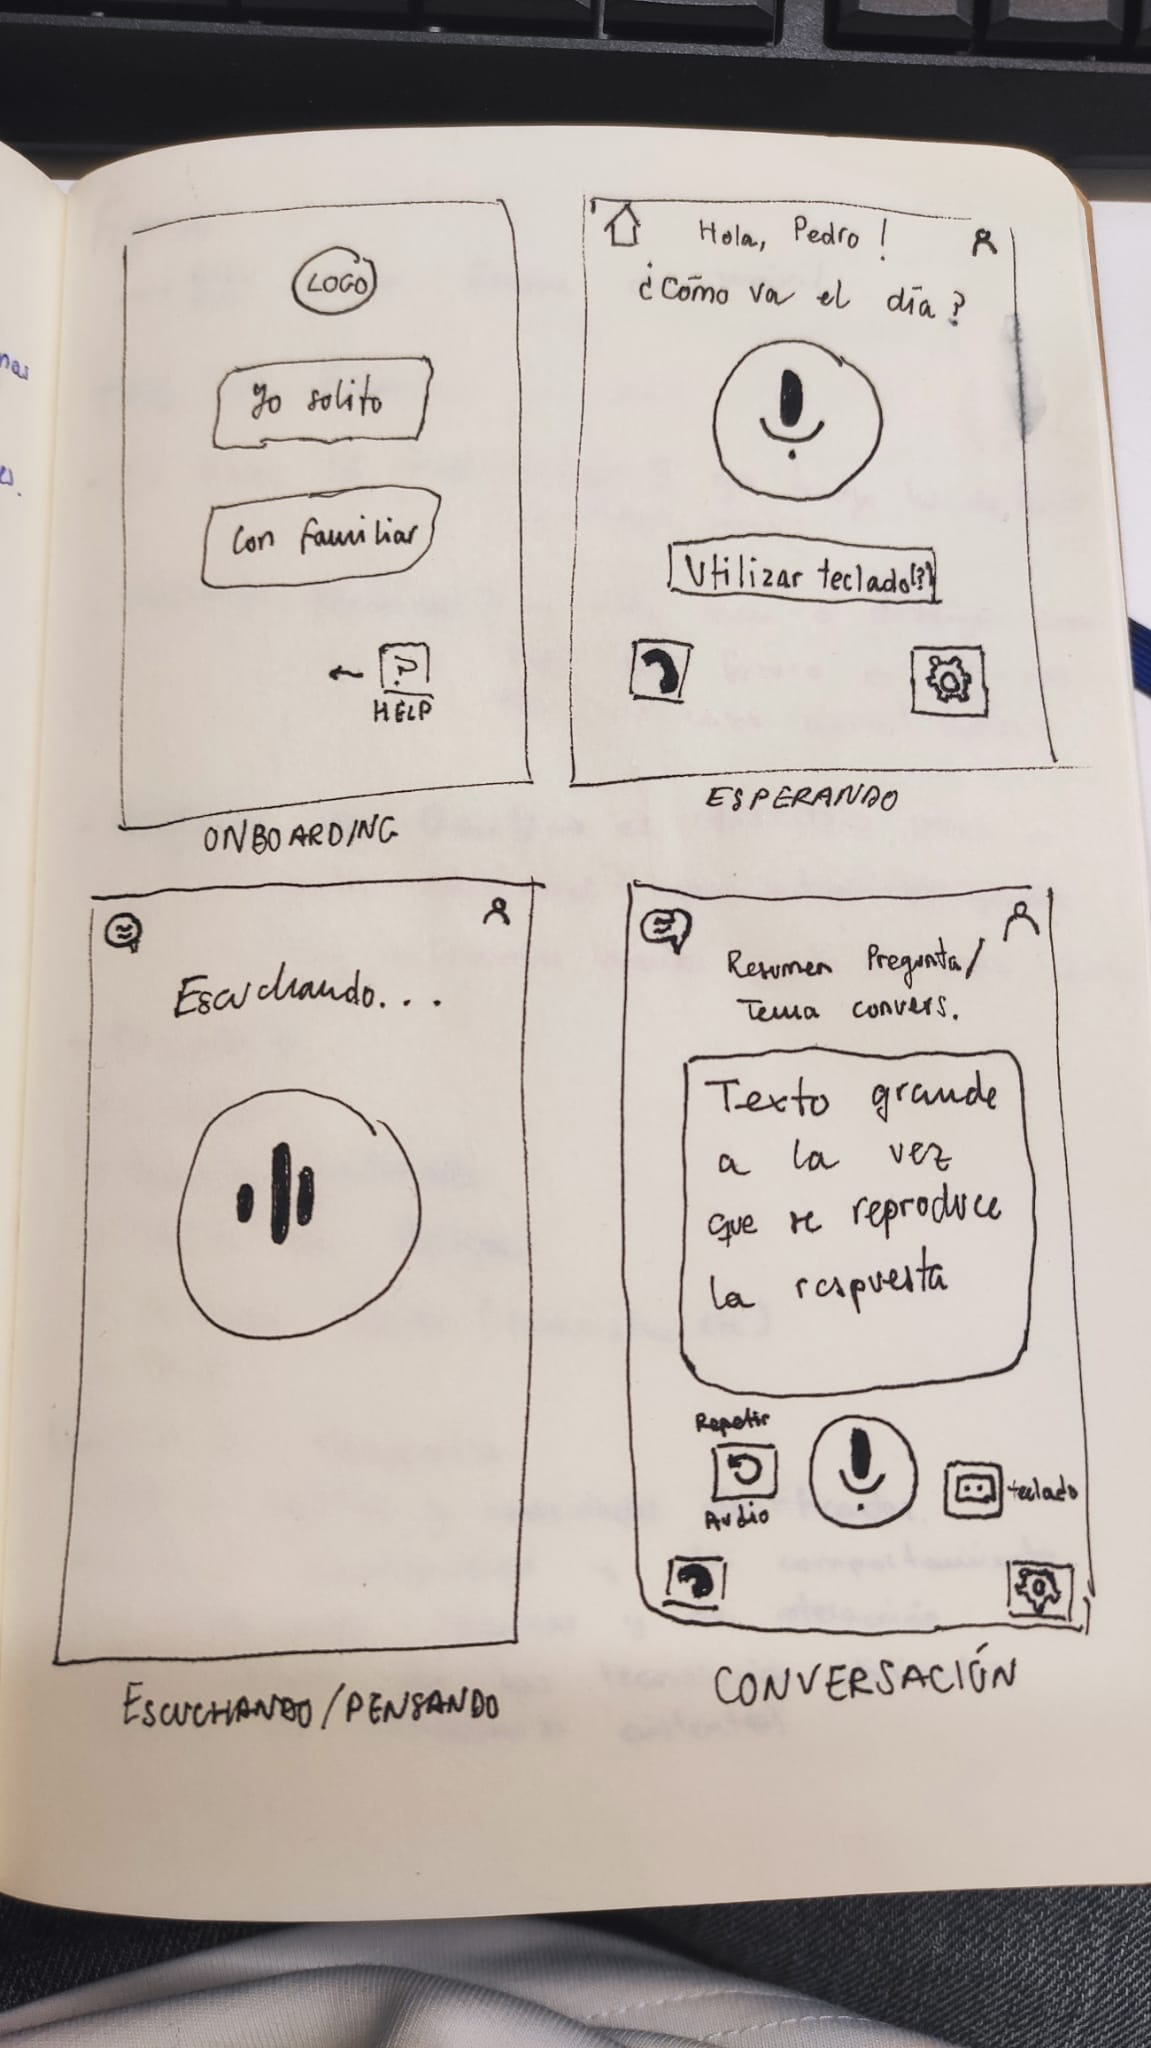
\includegraphics[height=11.5cm, trim={100 160 40 140}, clip]{imagenes/bocetos/boceto_mano_generico.jpeg}
  \caption[Bocetos a mano de los cuatro estados de la interfaz del mayor.]{Bocetos iniciales a mano de los cuatro estados de la interfaz del mayor: selección de autonomía, espera, escucha y conversación.}
  \label{fig:boceto-libreta}
\end{figure}

\subsection{Wireframes en Canva}

\begin{figure}[!tbp]\centering
  \begin{subfigure}[t]{0.3\textwidth}\centering
    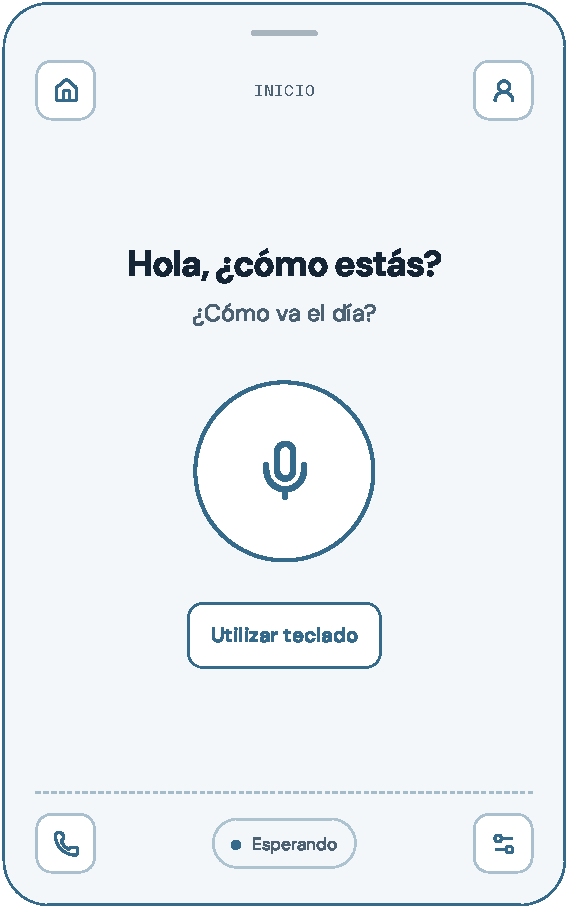
\includegraphics[width=\linewidth]{imagenes/bocetos/canva-1-inicio}
    \caption{Azul calmado}
  \end{subfigure}\hfill
  \begin{subfigure}[t]{0.3\textwidth}\centering
    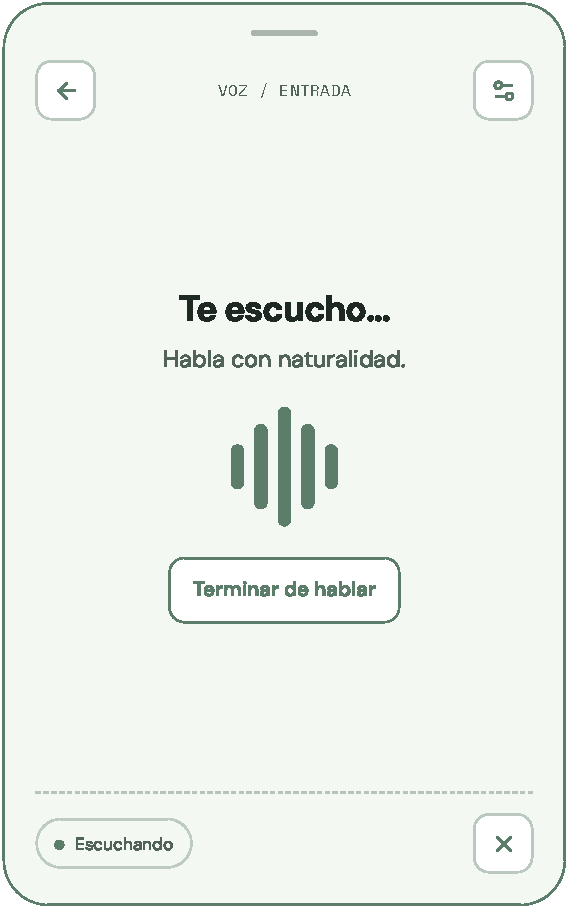
\includegraphics[width=\linewidth]{imagenes/bocetos/canva-2-escuchando}
    \caption{Verde salvia}
  \end{subfigure}\hfill
  \begin{subfigure}[t]{0.3\textwidth}\centering
    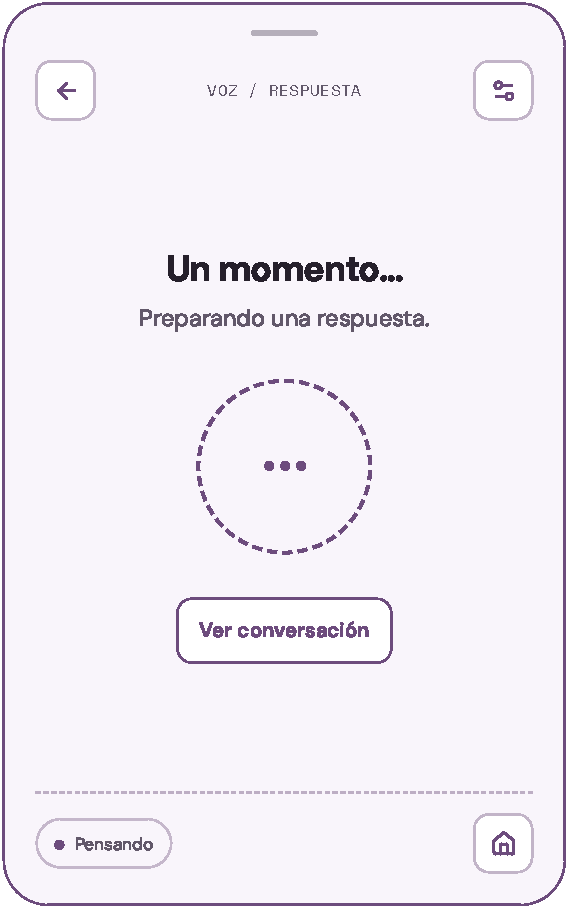
\includegraphics[width=\linewidth]{imagenes/bocetos/canva-3-procesando}
    \caption{Ciruela suave}
  \end{subfigure}

  \medskip
  \begin{subfigure}[t]{0.3\textwidth}\centering
    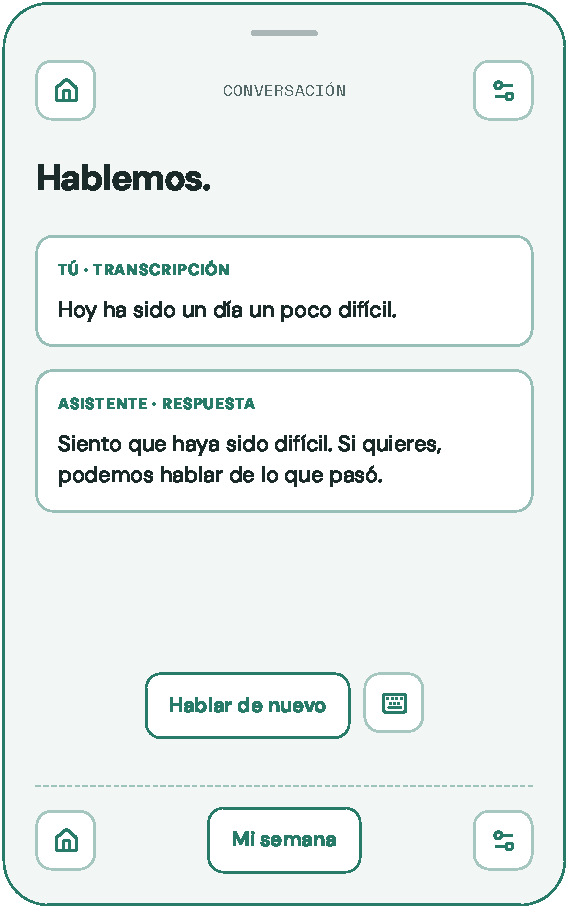
\includegraphics[width=\linewidth]{imagenes/bocetos/canva-4-conversacion}
    \caption{Azul petróleo}
  \end{subfigure}\hfill
  \begin{subfigure}[t]{0.3\textwidth}\centering
    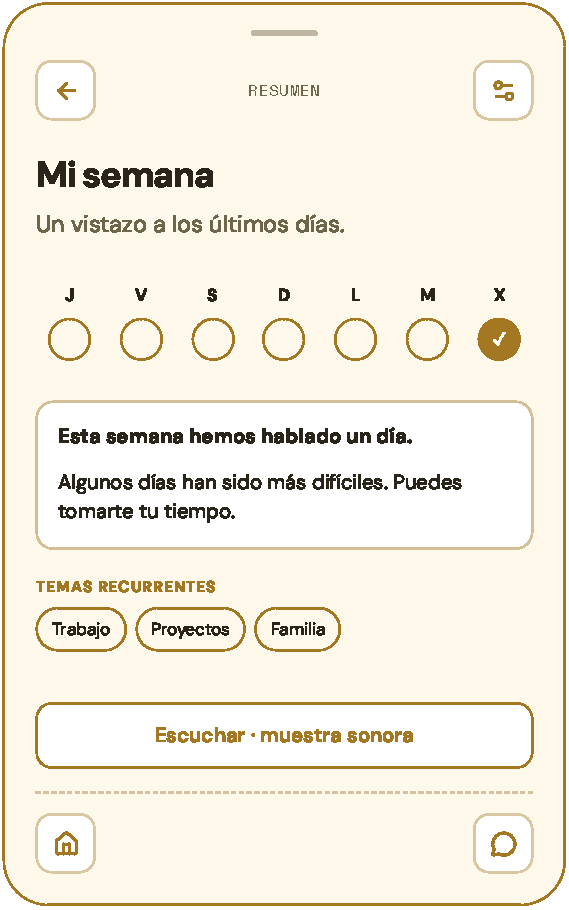
\includegraphics[width=\linewidth]{imagenes/bocetos/canva-5-mi-semana}
    \caption{Mostaza apagado}
  \end{subfigure}\hfill
  \begin{subfigure}[t]{0.3\textwidth}\centering
    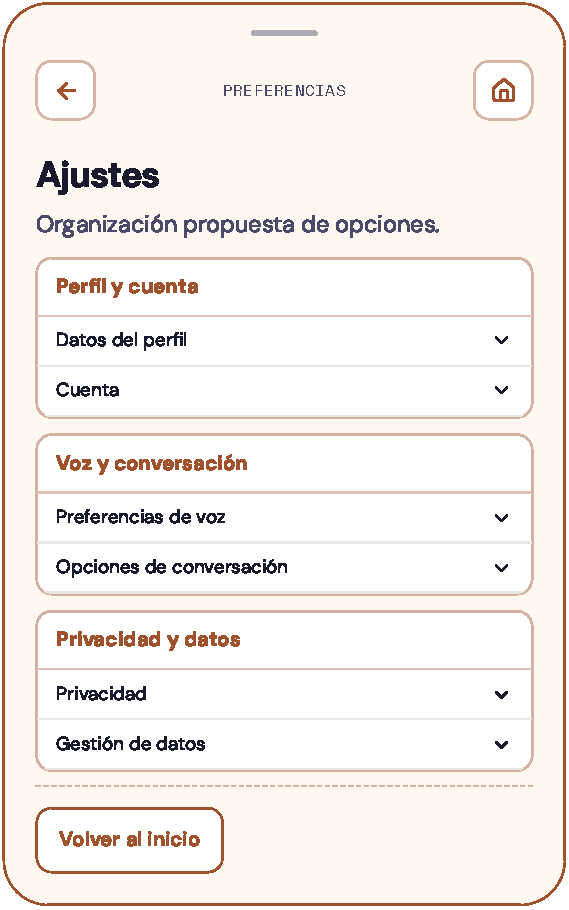
\includegraphics[width=\linewidth]{imagenes/bocetos/canva-6-ajustes}
    \caption{Canela, la elegida}
  \end{subfigure}
  \caption[Bocetos en Canva: una paleta candidata por pantalla.]{Bocetos en Canva del flujo del mayor (espera, escucha, procesamiento, conversación, <<Mi semana>> y Ajustes), cada pantalla con una de las paletas candidatas. La de Ajustes es la que adopta la aplicación.}
  \label{fig:bocetos-canva}
\end{figure}

La segunda etapa trasladó los bocetos supervivientes a wireframes digitales a escala, dibujados en Canva, y aportó la proporción: con las medidas reales, las restricciones de accesibilidad se ven como espacio ocupado. Un botón de 88~px de alto y un cuerpo de texto de 24~sp consumen enseguida la pantalla de un teléfono de gama media. El wireframe hace evidente que no caben seis opciones y obliga a decidir cuáles son las dos que importan.

La paleta de colores se decidió sobre una serie de bocetos en Canva que recorren el flujo completo del mayor, de la espera a Ajustes, con una paleta candidata distinta en cada pantalla y la misma composición en todas (\autoref{fig:bocetos-canva}). Se probaron cinco gamas (azul calmado, verde salvia, ciruela suave, azul petróleo y mostaza apagado) frente a la cálida, y se juzgaron con los dos criterios del apartado~\ref{sec:color}. El azul, el ciruela y el petróleo superan el 4{,}5:1 sobre su fondo, pero son tonos fríos, la zona del espectro que el cristalino envejecido filtra; el verde salvia (4{,}25:1) y la mostaza (3{,}82:1) no llegan a ese umbral. Solo Canela sobre blanco cálido cumple los dos, con 5{,}33:1.

\partesep{Parte II: Desarrollo}

\section{Stack tecnológico}
\label{sec:stack}

El sistema es una aplicación cliente Flutter (Dart, SDK \texttt{\textasciicircum 3.7.2}) compilada para Android (\code{minSdk} 24, \code{compileSdk} 36) apoyada en Firebase como \emph{Backend-as-a-Service}, en un conjunto de funciones propias desplegadas en Cloud Functions y en dos servicios de Google Cloud consumidos como API: Gemini, para la conversación y para el análisis de cada conversación al cerrarse, y Cloud Text-to-Speech, para la voz. La \autoref{tab:stack} recoge sus componentes.

\begin{table}[htbp]
    \centering
    \caption{Stack tecnológico en uso, con las versiones fijadas en \texttt{pubspec.yaml} y en el \texttt{package.json} de las funciones.}
    \label{tab:stack}
    \begin{tabularx}{\textwidth}{@{}l l >{\RaggedRight\arraybackslash}X@{}}
        \toprule
        \textbf{Capa} & \textbf{Componente} & \textbf{Función en el sistema} \\
        \midrule
        Cliente     & Flutter / Dart               & Interfaz nativa Android; sistema de diseño accesible propio \\
                    & \texttt{flutter\_riverpod} 2.5.1 & Estado reactivo e inyección de dependencias \\
                    & \texttt{go\_router} 17.0.0   & Enrutado declarativo con \emph{redirects} reactivos \\
                    & \texttt{speech\_to\_text} 7.3.0 & Transcripción de voz a texto (es-ES) \\
                    & \texttt{flutter\_tts} 4.2.5  & Síntesis de voz del dispositivo (respaldo) \\
                    & \texttt{just\_audio} 0.10.6  & Reproducción del audio sintetizado en la nube \\
                    & \texttt{url\_launcher} 6.3.2 & Apertura del marcador del sistema (emergencia) \\
                    & \texttt{permission\_handler} 12.0.1 & Permiso de micrófono \\
        \midrule
        Backend     & \texttt{firebase\_core} 3.15.2 & Inicialización del SDK \\
                    & \texttt{firebase\_auth} 5.7.0  & Autenticación dual (Google o anónima / correo) \\
                    & \texttt{google\_sign\_in} 7.2.0 & Selector de cuentas de Google del mayor \\
                    & \texttt{cloud\_firestore} 5.6.0 & Persistencia y sincronización en tiempo real \\
                    & \texttt{cloud\_functions} 5.4.0 & Cliente de las cinco \emph{callables} \\
                    & Cloud Functions (Node 22, gen 2) & Lógica de servidor (\autoref{tab:callables}) \\
        \midrule
        Servicios   & Vertex AI (\texttt{@google/genai}) & Gemini \texttt{gemini-2.5-flash} en el servidor: conversación, análisis y memoria \\
                    & Cloud Text-to-Speech           & Cuatro voces Chirp~3:~HD en español, a elegir \\
        \bottomrule
    \end{tabularx}

\end{table}

Las cuatro elecciones principales responden a dos restricciones: un único desarrollador con plazo ajustado y alta carga de trabajo, y un usuario cuyas limitaciones exigen controlar la interfaz por completo.

\textbf{Flutter} permite mantener una sola base de código, en lugar de una por plataforma, y dibuja su propia interfaz sin depender de los componentes del sistema operativo, que es lo que exige un sistema de diseño accesible redefinido por completo. Una aplicación web habría compartido la primera ventaja, pero con un acceso al micrófono más limitado. iOS es una plataforma posible pero no verificada.

\textbf{La inteligencia conversacional se delega en un LLM en la nube}, Gemini \code{gemini-2.5-flash}. Un modelo local exigiría inferencia neuronal a los terminales de gama media y baja a los que se dirige la aplicación, y ajustar un modelo propio era inviable sin datos conversacionales. Gemini comparte proyecto y facturación con Firebase y Cloud Text-to-Speech, tiene un coste despreciable a la escala de las pruebas (apartado~\ref{sec:costes}) y admite la invocación de funciones, con la que el asistente guarda el nombre del mayor en cuanto lo oye. El tono empático se consigue con la instrucción de sistema y los filtros de seguridad que fija en el servidor la función \code{chatTurn}.

\textbf{Firebase} resuelve lo que un desarrollador único no podría construir y operar a la vez: autenticación, persistencia y, sobre todo, la sincronización en tiempo real entre el dispositivo del mayor y el de su familiar, sin la que el modelo dual no existe. Sus \emph{streams} de documento son además la base de la fuente única de verdad (apartado~\ref{sec:ssot}). Donde el cliente no basta, el BaaS se completa con funciones propias (apartado~\ref{sec:paas}).

\textbf{Riverpod} cubre con un solo mecanismo el estado reactivo y la inyección de dependencias, y su \code{StreamProvider} encaja con los \emph{snapshots} de Firestore; la combinación habitual de BLoC con un localizador de servicios exige dos piezas para lo mismo. Se mantiene en la línea 2.x por un conflicto de la 3.x con \code{scheduleNewFrame} en el entorno de desarrollo Linux empleado, y todo el ecosistema FlutterFire se alinea sobre \code{firebase\_core} 3.x para evitar conflictos de dependencias transitivas: ambas fijaciones persiguen la reproducibilidad del \emph{build}.

\section{Arquitectura}
\label{sec:arquitectura}

\subsection{Visión general del sistema}
\label{sec:arquitectura-general}

La \autoref{fig:arquitectura} sitúa las piezas del sistema y cómo se comunican. Cada número de la figura identifica un flujo y cada letra, el orden de sus pasos; la flecha parte de quien inicia la operación.

El mayor y el familiar ejecutan la misma aplicación, que se comporta de una u otra forma según el rol almacenado en el perfil (revelación progresiva). Ambos se autentican contra Firebase Authentication (flujo~1), el mayor con su cuenta de Google o sin registrarse y el familiar con correo y contraseña, y ambos observan la colección \code{users} de Cloud Firestore (flujo~7), que actúa como memoria compartida entre los dos dispositivos y como mecanismo de propagación en tiempo real de las preferencias.

El ciclo conversacional ocupa los flujos~2 y~3. La voz la transcribe el reconocedor del propio Android, y la aplicación recibe solo el texto: no graba ni guarda el audio. El texto viaja a la \emph{callable} \code{chatTurn}, que lee del perfil el nombre del mayor y, si ha consentido guardar sus conversaciones, su memoria, y pide la respuesta a Gemini a través de Vertex AI; si el mayor dice cómo se llama, es la propia función quien guarda el nombre. La respuesta se trocea en frases, y cada una se envía a la \emph{callable} \code{synthesizeSpeech}, que llama a la API de Cloud Text-to-Speech con la voz elegida por el mayor y devuelve el audio. El reproductor del cliente lo reproduce con el volumen y la velocidad configurados y, si la síntesis de una frase falla o tarda demasiado, esa frase y las siguientes las pronuncia el motor de voz del dispositivo. Cuando el mayor prefiere escribir, el texto tecleado ocupa el lugar de la transcripción y la cadena es la misma, salvo que la respuesta solo se lee si él lo pide (apartado~\ref{sec:teclado}).


Al cerrarse cada conversación (flujo~4), el cliente entrega lo hablado a \code{closeConversation}, que comprueba en el perfil el consentimiento y el plazo de conservación, lo analiza con Gemini, guarda únicamente el resultado y descarta el texto. Ese resultado llega después a los dos dispositivos por Firestore, como cualquier otro dato. El emparejamiento (flujo~5) no se resuelve contra Firestore desde el cliente, sino a través de la \emph{callable} \code{validateAndLink}, que localiza al mayor por su código con credenciales de administrador y actualiza ambos perfiles en una única transacción. Y el consentimiento del mayor sobre sus conversaciones (flujo~6) solo puede escribirse a través de \code{setConversationConsent}. La llamada de emergencia (flujo~8), en cambio, no atraviesa el \emph{backend} en absoluto: construye un URI \code{tel:} y cede el control al marcador del sistema operativo. Por último, las reglas de seguridad de Firestore, la banda vertical de la figura, se interponen en todo acceso de cliente a la base de datos, de manera que ni siquiera un binario modificado puede leer o escribir fuera de lo que esas reglas permiten.


\afterpage{%
\begin{landscape}
\begin{figure}[p]\centering
  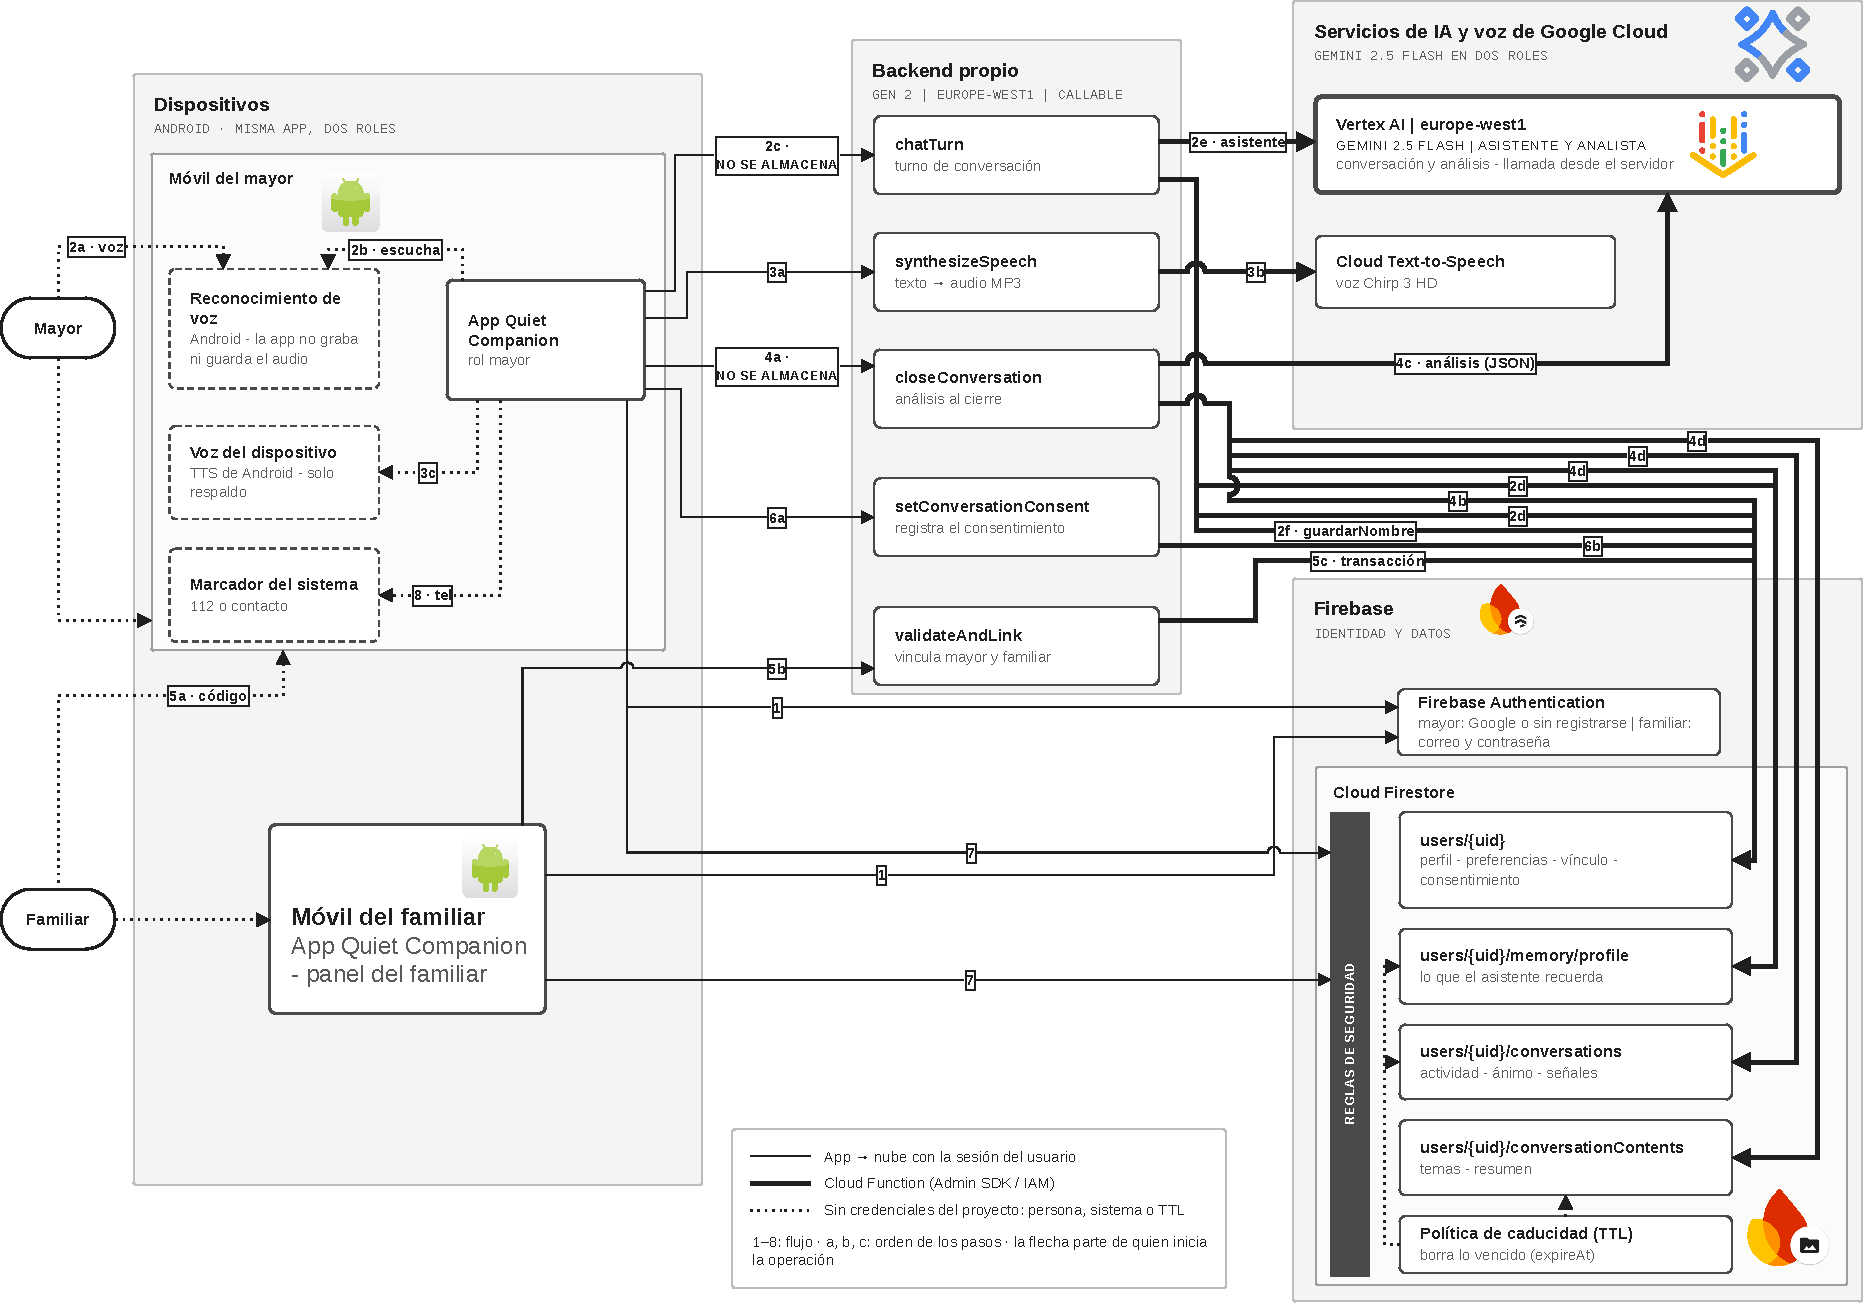
\includegraphics[width=\linewidth, height=\dimexpr\textheight-3\baselineskip\relax, keepaspectratio]{imagenes/arquitectura/arquitectura_sistema.pdf}
  \caption{Arquitectura del sistema: dispositivos, servicios gestionados y flujos de datos.}
  \label{fig:arquitectura}

  \vspace{2pt}
  {\footnotesize Fuente: Elaboración propia.}
\end{figure}
\end{landscape}}

Los servicios de pago, Gemini y Cloud Text-to-Speech, solo se alcanzan a través del \emph{backend} propio, de modo que el teléfono no guarda credenciales de ninguno de ellos; lo que el teléfono resuelve por sí solo, el reconocimiento de voz, la voz de respaldo y la llamada de emergencia, no sale de él; y el resto es acceso directo a Firestore, acotado por las reglas (apartado~\ref{sec:seguridad}).


\subsection[El servidor como plataforma gestionada: Firebase y Cloud Functions]{El servidor como plataforma gestionada: Firebase y\\ Cloud Functions}
\label{sec:paas}

Que el sistema tenga servidor propio no significa que el proyecto opere un servidor. Gracias a esa diferencia, un único desarrollador puede tener un \emph{backend} con lógica propia. El NIST define la plataforma como servicio (PaaS) como la capacidad de desplegar en la infraestructura del proveedor aplicaciones propias, escritas con los lenguajes y herramientas que este admite, sin gestionar ni controlar la red, los servidores, el sistema operativo ni el almacenamiento subyacentes: el cliente controla solo la aplicación desplegada y, en su caso, la configuración del entorno que la aloja \citep{NIST800145}. Quiet Companion combina dos variantes de ese modelo. Firebase actúa como \emph{Backend-as-a-Service}: la autenticación y la base de datos se consumen ya construidas, a través del SDK del cliente. Cloud Functions es una plataforma de funciones (\emph{Function-as-a-Service}), la forma más acotada de PaaS, en la que la unidad de despliegue es una función que el proveedor ejecuta bajo demanda, escala desde cero instancias y factura por invocación, de modo que el desarrollador no administra máquina alguna \citep{Jonas2019}. En la segunda generación, que es la que usa el proyecto, cada función se construye con Cloud Build y se despliega como un servicio de Cloud Run \citep{FirebaseFunctionsVersions}.

Un BaaS basta mientras toda la lógica pueda vivir en el cliente, y hay tres cosas que un cliente no puede hacer por sí solo. La primera es \textbf{guardar un secreto}: cualquier credencial empaquetada en la aplicación puede extraerse del binario, y la síntesis de voz y el análisis necesitan credenciales de Google Cloud (RNF-8). La segunda es \textbf{actuar sobre datos ajenos sin abrirlos a todos}: las reglas de Firestore autorizan operaciones enteras y no ven las cláusulas de una consulta, de modo que lo que exige buscar o escribir fuera del documento propio, como la vinculación, solo es seguro con privilegios de servidor (RNF-9). La tercera es \textbf{dar fe}: la hora de un consentimiento, la comprobación de que existe antes de analizar nada o el tope del plazo de conservación no pueden depender de lo que declare un dispositivo que controla el propio usuario. Esas necesidades se traducen en funciones propias, y la \autoref{tab:callables} recoge las cinco que componen el \emph{backend}.

Las cinco funciones son \emph{callables} (\code{onCall}) y no funciones HTTP genéricas ni disparadores de base de datos: el SDK de Firebase adjunta y verifica el token de sesión en cada invocación, de modo que el servidor toma la identidad de quien llama de \code{request.auth} y nunca de un parámetro, y nadie puede pedir que se actúe en nombre de otro. Un disparador no servía para el análisis, porque habría exigido escribir antes la transcripción en Firestore. Todas se despliegan en \code{europe-west1}, junto a los datos, con un tope de diez instancias como salvaguarda de coste en un proyecto sin financiación, y ninguna maneja claves: se autentican ante Cloud Text-to-Speech y Vertex AI con las credenciales por defecto de la cuenta de servicio del entorno. La lógica que decide (validar la entrada, sanear la respuesta del modelo, aplicar los cambios de memoria o calcular cuándo caduca un dato) vive en módulos puros separados de los manejadores, y se prueba con \code{node --test} sin emulador ni red, en veintitrés casos. Los registros contienen longitudes e identificadores, nunca texto de una conversación.

\begin{table}[htbp]
    \centering
    \caption{Funciones del \emph{backend}, todas \emph{callables} desplegadas en \texttt{europe-west1}.}
    \label{tab:callables}
    \small
    \begin{tabularx}{\textwidth}{@{}l >{\RaggedRight\arraybackslash}X >{\RaggedRight\arraybackslash}X@{}}
        \toprule
        \textbf{Función} & \textbf{Qué hace} & \textbf{Por qué en el servidor} \\
        \midrule
        \texttt{chatTurn}               & Responde cada turno de la conversación y guarda el nombre del mayor cuando lo dice & Gemini sin clave; el servidor fija las instrucciones del asistente y solo lee la memoria si hay consentimiento \\
        \addlinespace
        \texttt{synthesizeSpeech}       & Convierte una frase en audio con la voz Chirp~3:~HD elegida & Las credenciales de Cloud TTS no salen del servidor, único que conoce los nombres de las voces \\
        \addlinespace
        \texttt{validateAndLink}        & Vincula mayor y familiar por el código, en una transacción & Busca por código con privilegios de administrador sin que \texttt{/users} sea enumerable \\
        \addlinespace
        \texttt{setConversationConsent} & Registra o retira el consentimiento del mayor & La hora del servidor es la prueba; programa el borrado de lo guardado \\
        \addlinespace
        \texttt{closeConversation}      & Analiza la conversación al cerrarse y actualiza la memoria & Gemini sin clave; la transcripción no se almacena; aplica los plazos \\
        \bottomrule
    \end{tabularx}

\end{table}


La mayor ventaja de la plataforma está en el proceso. Un cambio en el \emph{prompt} del análisis o en la voz se publica con \code{firebase deploy}, sin generar ni instalar una APK nueva, y cada análisis guarda la versión del \emph{prompt} que lo produjo. A cambio, la primera invocación tras un periodo sin uso paga el arranque en frío de la instancia, que en la voz cubre el respaldo al motor del dispositivo, y el proyecto queda ligado a la plataforma de Google, una dependencia ya asumida al elegir Firebase.

\subsection{Estructura core/ y features/, y capas por \emph{slice}}

El código se organiza según el modelo híbrido Clean Feature-Sliced (CFS) prescrito por RNF-11: rebanadas verticales de funcionalidad sobre un núcleo transversal. Frente a la organización por capas técnicas, que reparte cada funcionalidad entre varias carpetas, CFS agrupa por funcionalidad; añade una regla explícita contra el acoplamiento lateral, y renuncia a las capas adicionales de Feature-Sliced Design estricto, desproporcionadas para el tamaño del proyecto. Dentro de cada rebanada se usa la nomenclatura de Clean Architecture, conocida por cualquier desarrollador.

\begin{lstlisting}[style=Consola, float=!tbp, caption={Estructura real del árbol de código fuente.}, label={lst:arbol}]
lib/
|-- core/                 # lo que comparten dos o más features
|   |-- config/           # router, redirect, filas de ajustes, plazos
|   |-- constants/        # firestore_paths
|   |-- models/           # usuario, consentimiento, conversación...
|   |-- providers/        # currentUserProvider, linkedElderProvider...
|   |-- repositories/     # autenticación, conversaciones y memoria
|   |-- services/         # Gemini, voz (STT y TTS), cierre...
|   |-- theme/            # AppTheme
|   |-- utils/            # sentence_splitter, week_summary
|   `-- widgets/          # ElderButton, SignOutButton
|-- features/
|   |-- conversation/  {data, domain, presentation}
|   |-- dashboard/     {domain, presentation}
|   |-- emergency/     {presentation}
|   |-- my_week/       {domain, presentation}
|   |-- onboarding/    {domain, presentation}
|   |-- privacy/       {data, domain, presentation}
|   `-- settings/      {presentation}
`-- main.dart, firebase_options.dart
functions/                # index.js (5 callables) y lógica pura
firestore.rules, firestore-tests/
\end{lstlisting}

Una \emph{feature} no importa nunca de otra, es decir, no hay acoplamiento horizontal, y lo compartido va a \code{core/}. El único punto de \code{core/} que conoce las \emph{features} es el enrutador, que compone sus pantallas.

Un ejemplo claro es \code{settings\_rows.dart}. Las filas de la pantalla de ajustes viven en \code{core/config/} y no en \code{features/settings/}, aunque intuitivamente pertenezcan a esa \emph{feature}, porque las consumen dos \emph{features} que no pueden acoplarse entre sí: \code{conversation} decide con ellas si muestra el botón de Ajustes, y \code{settings} decide qué muestra. Ubicar la lista en cualquiera de las dos habría obligado a la otra a importarla. Por la misma razón, la agregación semanal que muestran el panel del familiar y <<Mi semana>> vive en \code{core/utils/week\_summary.dart}, y el repositorio de autenticación, que usan el \emph{onboarding}, el panel, Ajustes y el contacto de emergencia, en \code{core/repositories/}.

\code{emergency} y \code{settings} tienen solo \code{presentation} porque su lógica se resuelve con servicios de \code{core/} y funciones puras, sin estado propio, y una carpeta \code{domain} vacía por simetría sería complicarlo sin necesidad.

\subsection{Single Source of Truth: \texttt{currentUserProvider}}
\label{sec:ssot}

Varias partes del sistema necesitan el documento \code{users/{\char123}uid{\char125}} en tiempo real: el enrutador para decidir redirecciones, la pantalla principal para el tamaño de letra, el servicio de voz para el volumen y la velocidad, y el panel del familiar. Que cada uno abriese su propia suscripción a Firestore duplicaría escuchas y repartiría la responsabilidad de mantener el dato.

La arquitectura adopta un \textbf{único punto de escucha}. \code{firebaseAuthUserProvider} emite el usuario de Firebase Auth; \code{currentUserProvider} lo observa y, cuando hay sesión, se suscribe a \code{users/{\char123}uid{\char125}} y lo mapea a \code{UserModel}. Cualquier widget o controlador, en cualquier punto de la aplicación, se limita a observar ese proveedor con \code{ref.watch}, y Riverpod reconstruye solo a quienes lo observan cuando Firestore emite.

Cuando el familiar completa el emparejamiento, la transacción borra el \code{linkCode} del documento del mayor; el \emph{stream} emite, el enrutador recalcula su decisión y el dispositivo del mayor avanza solo a la pantalla siguiente, sin que el mayor pulse nada. El mismo mecanismo propaga en caliente, sin código adicional, las preferencias de accesibilidad (RF-6).

El panel del familiar aplica el mismo patrón al documento del mayor: \code{linkedElderProvider} es para el familiar lo que \code{currentUserProvider} es para el propio usuario. El panel pinta desde ese \emph{stream} y cada control escribe solo su campo, con una ruta de punto (\code{preferences.volume}), nunca el documento entero. Es lo que permite que el mayor y su familiar modifiquen el mismo documento sin pisarse: el mayor ajusta sus escalas y el asistente aprende su nombre, y ningún deslizador del familiar puede revertirlo. Cada deslizador escribe en \code{onChangeEnd}, una vez por gesto y no decenas de veces por segundo, y la actualización es optimista: si la escritura falla, la propia caché de Firestore devuelve el control a su valor real, en lugar de dejar en pantalla uno que nunca llegó a guardarse.

\subsection{Gestión de estado e inyección de dependencias}
\label{sec:estado-di}

Todo estado de negocio se modela como un \code{StateNotifier} sobre una clase de estado inmutable con \code{copyWith}. No se usa \code{setState} para lógica de negocio en ningún punto; las pantallas son \code{ConsumerWidget} o \code{ConsumerStatefulWidget} que observan y dibujan. El único estado local admitido en la capa de presentación es el estrictamente efímero de un widget: la posición de un deslizador mientras se arrastra, la posición de un \code{ScrollController}.

Riverpod cubre simultáneamente el estado reactivo y la inyección de dependencias (RNF-12): servicios y repositorios se resuelven vía \code{Provider} y se pasan por constructor, nunca se instancian dentro de la clase que los usa. Gracias a ello, los tests de la pantalla de emergencia sustituyen \code{TtsService}, \code{SpeechService} y \code{EmergencyCallService} por falsos sin tocar los \emph{plugins} reales, y el controlador del chat recibe todos sus servicios por constructor.

\subsection{Operaciones atómicas y enrutado reactivo}

El emparejamiento entre mayor y familiar exige modificar dos documentos de usuarios distintos sin que pueda quedar un estado intermedio en el que uno esté vinculado y el otro no. Se resuelve con una transacción de Firestore, ejecutada en el servidor dentro de \code{validateAndLink} (apartado~\ref{sec:seguridad}), que revalida el código y actualiza ambos documentos en una sola operación. Es una transacción y no un lote de escritura (\code{WriteBatch}) porque necesita \emph{leer}: el contacto de emergencia del familiar se copia al mayor solo si este no ha fijado uno a mano, y eso exige leer antes su documento.

\code{RouterNotifier} observa los dos controladores de autenticación, el estado de Firebase Auth y \code{currentUserProvider}, y notifica a \code{go\_router} en cada cambio para que recalcule la redirección. La decisión de destino se toma sobre el dato en vivo del proveedor, con el estado del controlador únicamente como respaldo durante el intervalo previo a la primera emisión del \emph{stream}, y una guarda de rol impide que el documento de un familiar se use para decidir la ruta de un mayor. Esa decisión vive en una función pura, \code{routeRedirect}, extraída para que las pruebas del enrutador cubran la lógica real y no una copia escrita a mano. La misma función envía a \code{/consent}, antes de la pantalla principal, al mayor ya dado de alta que nunca ha respondido a la pregunta del consentimiento (apartado~\ref{sec:privacidad}).

\section{Seguridad: identidad, vinculación y reglas}
\label{sec:seguridad}

La seguridad del sistema descansa en tres piezas: cómo se identifica cada actor, cómo se vinculan mayor y familiar sin exponer a terceros, y qué reglas protegen cada acceso a la base de datos.

\textbf{Autenticación dual.} El familiar usa correo y contraseña, porque necesita una cuenta portable. Al mayor, escribir un correo y una contraseña le supondría una barrera real, así que la bienvenida le ofrece dos vías del mismo peso: \textbf{su cuenta de Google}, que se elige sin escribir nada, o \textbf{entrar sin registrarse}, con una sesión anónima. Ni el perfil ni las reglas distinguen cómo ha entrado, porque las dos vías dan un identificador de Firebase del mismo tipo. La sesión anónima no ofrece cierre de sesión, porque cerrarla o reinstalar la aplicación generaría un identificador nuevo y perdería el perfil; por eso <<Mi cuenta>> permite guardarla después con Google sin cambiar de identificador, y la memoria, las conversaciones y el vínculo con el familiar se conservan. La cuenta de Google de un familiar no sirve para entrar como mayor: la aplicación cierra la sesión antes de que elegir modo le reescriba el rol.

\textbf{Vinculación en el servidor.} El mayor que elige el modo vinculado recibe un código de cuatro caracteres, sin símbolos confundibles, que su familiar introduce en su propia aplicación. Encontrar al mayor a partir de ese código es una consulta de colección (\code{where('linkCode', '==', code)}), y las reglas de Firestore no ven las cláusulas de una consulta: solo pueden permitir o denegar la operación entera. Si la búsqueda se hiciera desde el cliente, \code{/users} tendría que ser consultable por cualquier usuario autenticado, y cualquiera con la aplicación instalada podría enumerar el directorio de usuarios, con sus nombres y sus teléfonos de contacto. Por eso la vinculación es una \emph{callable}, \code{validateAndLink}. La búsqueda corre con credenciales de administrador, lo que permite denegar a todo cliente el listado de \code{/users}; el identificador del familiar lo toma el servidor de la sesión autenticada y no de un parámetro, así que nadie puede vincular a un tercero; el servidor comprueba que quien vincula es realmente un familiar registrado; y el código se consume dentro de la misma transacción que lo valida, por lo que solo sirve una vez. Así se cumple RNF-9.

\textbf{Reglas que modelan el código real.} Las reglas de Firestore describen operación por operación lo que hace la aplicación: lectura solo por identificador, para el dueño y para el familiar vinculado; borrado siempre denegado; escritura del familiar acotada por campo a las preferencias, el nombre y los plazos de la conversación, de modo que el panel no puede cambiar el rol del mayor, romperle el vínculo, reescribirle el contacto de emergencia ni decidir sobre su consentimiento; y denegación por defecto para todo lo demás. Las reglas no admiten nada que la aplicación no haga: si una operación cambia y las reglas no la contemplan, se muestra un error y las pruebas lo señalan, en vez de que las reglas queden desfasadas sin que nadie lo note.

\textbf{Reglas verificadas contra el emulador.} Cuando una regla falla, el error aparece en el dispositivo del usuario y no en el del desarrollador. Por eso se prueban contra el emulador de Firestore, con doce casos agrupados por sujeto (el dueño, el familiar vinculado y un autenticado cualquiera) y por garantía (que \code{/users} no sea enumerable, que el consentimiento y el análisis solo los escriba el servidor y que el familiar vea solo lo que el mayor elige). Son las únicas pruebas del proyecto que comprueban lo que el sistema debe rechazar a quien no usa la aplicación.

\textbf{Ninguna credencial en el teléfono.} La conversación en vivo pasa por \code{chatTurn}, que llama a Gemini a través de Vertex AI con las credenciales de la cuenta de servicio, igual que el análisis al cierre, de modo que el binario no contiene credenciales de ningún servicio de pago y RNF-8 se cumple. La función compone además las instrucciones del asistente y sus filtros de seguridad, que un cliente modificado no puede sustituir, y acota la longitud de cada turno y del historial que recibe. El precio es un salto de red más por turno en el camino que más se usa, el de la respuesta en vivo.


\section{La voz}
\label{sec:voz}

La voz es la interfaz primaria del mayor, y de su calidad, su ritmo y su turno depende que la conversación resulte natural.

\textbf{Síntesis en la nube.} El motor de voz nativo de Android produce una voz perceptiblemente robótica, cuya calidad depende además del motor instalado en cada dispositivo, y para una población mayor una voz poco natural reduce la inteligibilidad y la disposición a conversar. Por eso la voz se sintetiza en el servidor, con Cloud Text-to-Speech y las voces Chirp~3:~HD en español de España, del mismo proveedor que el resto del sistema. Dos mecanismos la hacen viable en una conversación: el \textbf{troceado por frases}, que sintetiza la primera oración y la reproduce mientras se sintetiza la siguiente, de modo que el primer audio llega tras un solo viaje de red; y el \textbf{respaldo sin reintentos}: si la síntesis de una frase falla o tarda, esa frase y las siguientes se pronuncian con el motor del dispositivo, porque para este usuario una voz peor pero inmediata es preferible a un silencio imprevisible.

\textbf{Una voz a elegir.} El mayor elige entre cuatro, dos de mujer y dos de hombre: las del catálogo Chirp~3:~HD que Google describe con el registro de un acompañante (cálida, dulce, amable y suave). No son más porque se comparan de oído, y con más opciones ya no se recuerda cómo sonaba la primera. Cada una se presenta por cómo suena (<<Voz de hombre, amable>>) y no por su nombre de catálogo, y al tocarla se guarda y dice una frase de muestra, sin botón de guardar, como las escalas. El familiar puede elegirla también desde el panel, tras escuchar cada opción. La voz por omisión es masculina porque, en los terminales probados, el motor del dispositivo habla con voz de mujer, y así el respaldo se reconoce de oído.

\textbf{Preferencias aplicadas en el reproductor.} La función de síntesis recibe solo el texto y la clave de la voz, que traduce a su nombre real desde una lista cerrada: una clave desconocida suena con la voz por omisión, y nadie puede pedir una voz cualquiera ni colar parámetros de síntesis. Sintetiza siempre a ritmo neutro. El volumen y la velocidad elegidos los aplica el reproductor del cliente, con el mismo factor de conversión que \code{flutter\_tts} usa en Android, y así el ajuste significa lo mismo con la voz de la nube y con la de respaldo. \code{just\_audio} sirve el audio en memoria a través de un servidor HTTP local en \code{127.0.0.1}, y como Android prohíbe por defecto el tráfico en claro, la configuración de seguridad de red lo permite exclusivamente hacia esa dirección y no de forma global.

\textbf{Escucha por turnos.} El reconocedor de voz de Android corta su sesión en cada pausa, así que la aplicación encadena sesiones y da el turno por terminado tras un silencio, sin que el mayor tenga que pulsar nada. Cuánto silencio basta depende de la persona, que puede detenerse a pensar a mitad de una idea. Por eso no es una constante sino una escala más de Ajustes, <<Tiempo que te espero>>, de dos a diez segundos y tres por omisión. Al cerrar cada sesión, la aplicación espera, con un tope de un segundo, al resultado final del reconocedor, porque Android avisa de que ha dejado de grabar antes de entregar el único resultado que contiene la última palabra.

\section{Conversación, memoria y seguimiento del bienestar}
\label{sec:conversacion}

Resumir una conversación, medir el ánimo o recordar exigen decidir antes qué es \emph{una conversación}. Sin una frontera, la sesión del modelo duraría lo que la aplicación abierta: con el teléfono encendido en un soporte, abarcaría la charla de la mañana y la de la noche, con un historial que crecería sin límite y se reenviaría entero en cada turno. Este apartado recorre las cuatro piezas que resuelven HU-5 y HU-6: la frontera de la conversación, su análisis al cerrarse, la memoria que de él se deriva y la presentación del resultado al mayor y a su familiar. En ninguna de las cuatro se almacena la transcripción.

\subsection{La conversación como unidad}

Una conversación empieza con el primer turno del mayor y termina con lo primero que ocurra de dos cosas: que pase un tiempo sin turnos, cinco minutos por omisión, contado desde que el asistente \emph{termina} de hablar para que una respuesta larga no consuma la ventana, o que la aplicación pase a segundo plano. Si el mayor sale hacia el marcador de emergencia, la conversación sigue abierta. No hay botón de <<terminar>>, porque sería una decisión más para el mayor y nadie da por terminada de forma explícita una charla con quien le acompaña, de modo que las conversaciones no se cerrarían nunca.

Mientras dura, la conversación vive solo en la memoria del teléfono: el controlador del chat acumula los turnos completos, con su autor y su hora, y excluye las respuestas de error de la propia aplicación, que no son conversación y sesgarían el análisis hacia lo negativo. Al cerrarse, el controlador entrega ese búfer al servidor sin que el mayor espere ni vea nada, lo vacía y deja preparada una sesión nueva del modelo para el turno siguiente. Si el mayor ha intervenido menos de tres veces, solo sale del dispositivo la constancia de la conversación, sin texto, porque un <<hola, adiós>> no tiene ánimo que medir. Y la escucha del ciclo de vida de la aplicación vive en el proveedor del chat y no en una pantalla, para que la conversación se cierre aunque el mayor esté en Ajustes al salir.

Si Android mata el proceso antes de que el envío llegue al servidor, el análisis de esa conversación se pierde. Guardar el búfer en disco para sobrevivir a esa muerte dejaría la transcripción en reposo en el dispositivo, justo lo que el diseño prohíbe. Como efecto secundario favorable, que la sesión del modelo coincida con la conversación acota el coste de cada turno, que deja de crecer con el tiempo que la aplicación lleve abierta.

\subsection{Análisis al cierre en el servidor}

Todo el análisis ocurre al cerrarse la conversación, en el servidor, por cuatro razones. Lo que no se guarda solo puede analizarse mientras existe, de modo que el análisis tiene que hacerse en el cierre. Analizar la transcripción, y no un resumen previo, es analizar las palabras del mayor y no una paráfrasis escrita para ser breve y neutra, en la que el afecto ya se ha perdido. Pasarla por una función propia que no la escribe no añade destinatario ni almacenamiento, porque la transcripción ya viaja a Google en cada turno. Y un \emph{prompt} en el servidor se ajusta sin publicar una APK nueva.

La realización es una sola \emph{callable}, \code{closeConversation}, que recibe la conversación terminada y hace una única llamada al modelo; la \autoref{fig:secuencia-cierre} recoge el recorrido completo. La función comprueba primero que quien llama es un mayor y que su consentimiento está vigente; si no lo está, rechaza la petición sin escribir nada, con independencia de que el cliente, que tampoco envía nada sin consentimiento, se haya comportado bien. Valida después la entrada, y cuenta ella misma los turnos del mayor en lugar de fiarse del número que declara el cliente. Y llama a \code{gemini-2.5-flash} a través de Vertex AI con \textbf{salida estructurada}: un esquema JSON con enumerados cerrados y temperatura baja, de modo que de una sola llamada salen a la vez el sentimiento, las señales, los temas, el resumen y los cambios de memoria. Tratar el texto una vez, y no una por dato, es también minimización. La respuesta se sanea antes de escribirse, porque lo que entra en la base de datos no puede depender de que el modelo cumpla el esquema <<casi siempre>>.

\begin{figure}[htbp]
    \centering
    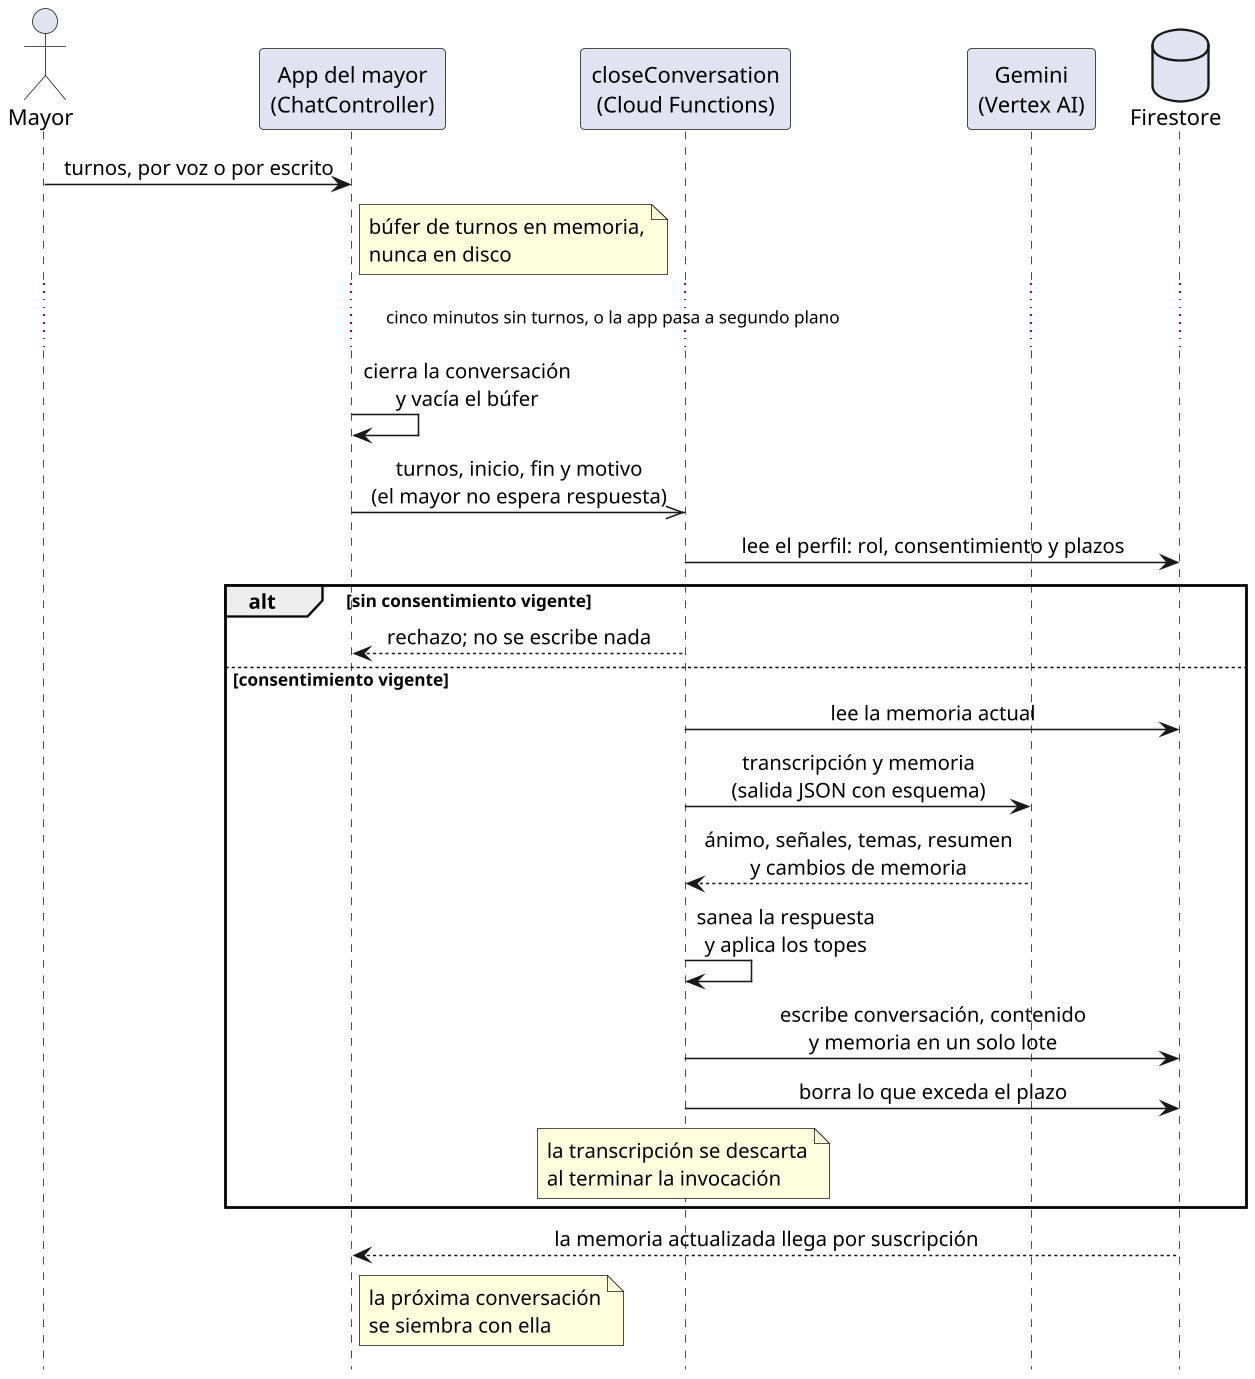
\includegraphics[width=0.85\textwidth]{imagenes/uml/secuencia_cierre.png}
    \caption{Cierre y análisis de una conversación: del búfer en memoria del teléfono a los documentos que se guardan, sin que la transcripción llegue a almacenarse.}
    \label{fig:secuencia-cierre}

    \vspace{2pt}
    {\footnotesize Fuente: Elaboración propia.}
\end{figure}

El análisis depende de los criterios del \emph{prompt}, que se versiona y queda registrado junto a cada resultado. El sentimiento es el del mayor y no el del diálogo, porque el asistente es cálido siempre y evaluar la conversación entera daría <<positivo>> casi siempre. Las clases son las tres de RF-8, sin escalas numéricas de valencia y activación que aparentarían una precisión que un modelo sin calibrar no tiene. Las señales salen de una lista cerrada de seis (soledad, tristeza, preocupación, malestar físico, desorientación y riesgo) y solo cuentan si las expresa el mayor, no si el asistente pregunta por ellas. El resumen ocupa una o dos frases en tercera persona, sin citas literales ni diagnósticos, y nombra a otras personas por su relación y no por su nombre. Y el \emph{prompt} advierte de que el texto procede de un reconocedor de voz, con sus errores. Si el modelo falla, la conversación se registra igualmente como actividad, con estado de fallo y sin reintentos, porque que el mayor hablase es un dato en sí mismo. El \autoref{lst:modelo-datos} muestra lo que se guarda, repartido en documentos que comparten identificador; el reparto lo impone el control de lo que ve el familiar, que se explica en el apartado~\ref{sec:privacidad}.

\begin{lstlisting}[style=Consola, caption={Lo que se guarda de cada conversación en Firestore. La transcripción no aparece en ninguno de los documentos.}, label={lst:modelo-datos}]
users/{elderId}/conversations/{id}         # "cómo me encuentro"
  startedAt, endedAt, elderTurns, endReason
  status:    analyzed | too_short | failed
  sentiment: positive | neutral | negative | null
  signals:   [loneliness, sadness, worry,
              physical_discomfort, confusion, risk]
  promptVersion, model, expireAt

users/{elderId}/conversationContents/{id}  # "de qué hablamos"
  endedAt, topics (máx. 5), summary, expireAt

users/{elderId}/memory/profile             # lo que recuerda
  facts (máx. 30), recent (3 últimos resúmenes), updatedAt
\end{lstlisting}

Las etiquetas de un modelo de lenguaje no están validadas clínicamente, de modo que se presentan como orientación y nunca como diagnóstico. Además, la señal de riesgo no convierte la aplicación en un sistema de alertas: el familiar la ve cuando abre el panel, y los avisos mediante notificaciones quedan como línea de trabajo futuro (apartado~\ref{sec:lineas-futuras}). La respuesta a una situación de crisis corresponde al chat en vivo, cuya instrucción de sistema incluye una regla explícita: responder con calma y sin quitarle importancia, animar a hablarlo con alguien de confianza y recordar el 024, la línea de atención a la conducta suicida, y el 112.

\subsection{La memoria del mayor}

Gemini no recuerda nada entre llamadas: el historial de la conversación es una lista de turnos en la memoria del teléfono, que el cliente reenvía entera a \code{chatTurn} en cada turno y que desaparece al terminar la conversación. Cualquier memoria entre conversaciones tiene que guardarse fuera y volver a entregarse al modelo. Se aprende al cerrar cada conversación, y no en vivo, porque solo se usa al empezar la siguiente. Aprenderla ahí es además gratis (no requiere otra llamada), porque la llamada del análisis ya lee la transcripción entera, y no añade latencia a lo único que el mayor percibe, la respuesta en vivo.

La misma llamada del cierre devuelve, por tanto, los cambios de la memoria y no un perfil reescrito: altas o correcciones por clave y claves que olvidar. Una lista de cambios explícitos se puede auditar, mientras que un perfil regenerado entero puede perder datos sin que nadie lo note. La función los aplica con topes estrictos, treinta datos en total y diez cambios por conversación con claves saneadas, y los guarda en un documento propio junto a los resúmenes de las tres últimas conversaciones. El \emph{prompt} excluye cualquier dato de salud, limita los datos de terceros a su nombre y su relación, y trata como borrado lo que el mayor pide olvidar.

Al empezar cada conversación, la sesión del modelo arranca con un bloque adicional en su instrucción de sistema, <<Lo que sabes de\ldots>> y <<De vuestras últimas conversaciones>>, acompañado de la indicación de usarlo con naturalidad, no recitarlo y no decir que se tienen notas; si la memoria está vacía, el bloque no aparece. La memoria llega al controlador del chat por suscripción y sin reconstruirlo, y una actualización nunca reinicia una conversación en curso: se aplica en la siguiente. Solo el nombre se aprende en vivo, mediante la función que el modelo invoca al oírlo, porque hace falta en la misma conversación. Es una forma ligera de generación aumentada por recuperación, sin infraestructura de búsqueda vectorial, que sería desproporcionada para treinta datos. La memoria va, por tanto, una conversación por detrás: lo que el mayor cuenta en una conversación se recuerda a partir de la siguiente.

\subsection{El seguimiento del bienestar: el panel del familiar y <<Mi semana>>}
\label{sec:bienestar}

El análisis tiene dos destinatarios: el familiar y el propio mayor. Si solo lo viera el familiar, al mayor independiente no le aportaría nada y al vinculado lo dejaría como objeto de seguimiento y no como destinatario de lo que se dice de él. Los dos ven los mismos datos en pantallas distintas, sin coste de arquitectura. Los modelos de lectura del análisis y la agregación semanal viven en \code{core/}, y la agregación es una función pura con pruebas, \code{summarizeWeek}, que calcula los días con conversación, el ánimo predominante, los temas más repetidos, los temas de las conversaciones con preocupación y el recuento de señales. Si cada pantalla calculara por su cuenta, el mayor y su familiar acabarían viendo números distintos. Lo que cambia entre ambas es la presentación.

El \textbf{panel del familiar} ordena sus secciones por fiabilidad: primero la actividad, que no depende de ningún modelo (cuándo habló por última vez, cuántos días y cuánto tiempo), y después las señales, el ánimo, los temas, la lista de conversaciones con su detalle y lo que el asistente recuerda. Todo lo que estima el modelo lleva el aviso <<Orientativo: lo estima un modelo de IA a partir de lo que dice. No es un diagnóstico>>. Si alguna conversación de la semana registró la señal de riesgo, el panel lo indica arriba y en rojo, con el 112 y el 024, que atiende también a familiares. Y si el mayor ha restringido lo que comparte, el panel lo explica en lugar de mostrar un error de permisos.

\textbf{<<Mi semana>>}, la pantalla del mayor, cuenta la semana con frases y no con gráficas, en segunda persona y en tono de refuerzo, con un botón <<Escuchar>> que las lee en voz alta (<<Esta semana hemos hablado 4 días>>, <<La mayoría de las veces te he notado bien>>). Una fila de siete días marca cuándo se habló y no cómo se encontraba cada día, porque busca reforzar y no evaluar. Las señales de soledad, tristeza o riesgo no se nombran nunca; de ellas solo aparece, suavizado, <<lo que más te ha rondado la cabeza>>. En caso de empate entre ánimos la agregación devuelve neutro: ante la duda, no se afirma ni que estuvo bien ni que estuvo mal. La pantalla indica, por último, qué parte de su análisis ve su familiar, con acceso directo para cambiarlo, así que <<Mi semana>> también le muestra lo que se guarda de él. El acceso aparece en la pantalla principal para todo mayor con el consentimiento activo y al menos una conversación analizada, sea independiente o vinculado. Las dos pantallas se recogen en el manual de usuario del apéndice~\ref{ap:manual}.

\section{Privacidad desde el diseño: el consentimiento informado}
\label{sec:privacidad}

De todo lo que hace el sistema, analizar las conversaciones de una persona mayor es lo más delicado, y es también lo que más lo separa de los compañeros conversacionales revisados en el capítulo~\ref{cap:marco-teorico}, uno de los cuales fue sancionado precisamente por carecer de base jurídica para tratar datos. Inferir el estado de ánimo o registrar molestias físicas puede revelar datos relativos a la salud, una categoría especial cuyo tratamiento el RGPD prohíbe salvo excepciones (art.~9.1), y la única realista para esta aplicación es el consentimiento explícito del interesado (art.~9.2.a) \citep{RGPD2016}. Este apartado explica cómo se ha diseñado ese consentimiento, cómo se hace cumplir y cómo se gobierna el plazo de conservación. Es un diseño conforme a los principios del Reglamento, no un dictamen jurídico.

\subsection{Quién consiente, cuándo y cómo}

El Reglamento define el consentimiento como una manifestación de voluntad libre, específica, informada e inequívoca, mediante una declaración o una clara acción afirmativa (art.~4.11), y precisa que el silencio, las casillas ya marcadas o la inacción no lo constituyen (considerando~32). Hace falta, por tanto, un gesto, y el diseño solo decide cuál. Para esta población es una pantalla propia con una sola pregunta, <<¿Quieres que guarde un resumen de nuestras conversaciones?>>, y dos botones del mismo tamaño, <<Sí, quiero>> y <<Ahora no>>, de modo que negarse cuesta exactamente lo mismo que aceptar. No es una casilla, porque una casilla de tamaño convencional incumpliría el área táctil mínima de RNF-2. Un botón <<Escuchar>> lee en voz alta la pregunta y su explicación, y <<Saber más>> abre la versión completa del texto.

Consiente siempre el mayor, en su propio dispositivo, también cuando está vinculado. Que consintiera el familiar no sería válido ni deseable porque, en esta aplicación, <<vinculado>> significa que al mayor le ayudan con la tecnología, no que exista una medida de apoyo que convierta al familiar en su representante, que sería paternalista. El familiar \textbf{ayuda a decidir}, el mayor \textbf{decide}. La pregunta aparece una sola vez y en el momento más temprano posible: justo después de elegir el modo independiente o justo después de completarse la vinculación, un momento que suele ser presencial, porque el familiar lee el código en la pantalla del mayor y puede explicarle la pregunta en persona. Se implementa como un paso del enrutador, y <<Ahora no>> también se registra, para no volver a preguntar.

El texto está en lenguaje llano y se ofrece en dos capas, una breve en la pregunta y otra completa en <<Saber más>>, en la línea de los artículos~12 y~13. Explica por separado qué se guarda (un resumen breve de cada conversación y cómo se ha sentido, nunca lo que dice palabra por palabra), qué se recuerda (lo que cuenta de su familia o de sus gustos, nunca nada de su salud), cómo se hace (lo hablado se envía a los servidores de Google, que lo analizan y no lo guardan), quién lo ve (su familiar, por su nombre, o solo él), cuánto tiempo se conserva y cómo puede retirarlo. El texto está versionado, y la versión leída se registra con la respuesta. Un único consentimiento cubre el análisis y la memoria, porque ambos sirven al propio mayor. Si está vinculado, la pregunta le dice además que su familiar verá cómo se encuentra y un resumen de lo que hablan, y el <<sí>> incluye ese nivel, que puede cambiar después en Ajustes. Y nada se trata hasta el <<sí>>: el consentimiento está desactivado por defecto, que es la protección de datos por defecto del artículo~25.2.

\subsection{Cómo se hace cumplir}

Un consentimiento que solo respeta la interfaz no protege nada, porque el familiar tiene sesión propia y podría leer cuanto las reglas le permitan, con esta aplicación o con otra. Por eso las tres garantías centrales se imponen en el servidor.

La primera es la prueba del consentimiento. El responsable debe poder demostrar que el interesado consintió (art.~7.1), y una hora tomada del dispositivo no demuestra nada. El registro del consentimiento, con la respuesta, la hora y la versión del texto leído, solo lo escribe \code{setConversationConsent}, con la hora del servidor; las reglas impiden que lo escriba cualquier cliente, incluido el propio mayor, y que un documento nazca con un consentimiento de serie. La función toma además la identidad de la sesión, de modo que un familiar no puede consentir por su mayor ni siquiera llamándola directamente.

La segunda es que sin consentimiento no se analiza nada. El cliente no envía la conversación si no lo hay, pero la garantía real es que \code{closeConversation} lo vuelve a comprobar y, si no está vigente, rechaza la petición sin escribir nada.

La tercera es qué ve el familiar. Hay tres niveles con nombre: <<Nada>>; <<Cómo me encuentro>>, que incluye la actividad, el ánimo y las señales; y <<Cómo me encuentro y de qué hablamos>>, que añade los temas, los resúmenes y la memoria. El <<sí>> del mayor vinculado fija el tercero, salvo que antes hubiera elegido otro, y a partir de ahí solo el mayor puede cambiarlo. Hacerlo cumplir tropieza con una limitación de Firestore, la de que las reglas no pueden filtrar campos, porque leer un documento es leerlo entero. Por eso cada conversación se reparte en dos documentos, y las reglas conceden la lectura de cada colección según el nivel. El \autoref{lst:reglas} muestra la función que lo decide.

\begin{lstlisting}[float=tbp, caption={Regla de lectura del familiar sobre el análisis del mayor (extracto de \texttt{firestore.rules}).}, label={lst:reglas}]
function companionMayRead(elderId, levels) {
  let elder = get(/databases/$(database)/documents/users/$(elderId)).data;
  return isSignedIn()
    && elder.get('linkedCompanionId', null) == request.auth.uid
    && elder.get('conversationConsent', {}).get('granted', false) == true
    && elder.get('companionSharing', 'none') in levels;
}

match /users/{userId} {
  match /conversations/{id} {             // cómo me encuentro
    allow read: if isOwner(userId)
      || companionMayRead(userId, ['wellbeing', 'full']);
    allow write: if false;                // solo el servidor
  }
  match /conversationContents/{id} {      // de qué hablamos
    allow read: if isOwner(userId)
      || companionMayRead(userId, ['full']);
    allow write: if false;
  }
}
\end{lstlisting}

La condición se evalúa al leer y no se copia al escribir: al bajar el nivel se oculta al instante también todo el historial. Las pruebas contra el emulador lo comprueban: un familiar con nivel <<Cómo me encuentro>> que intenta leer los resúmenes es rechazado, y uno cuyo mayor ha retirado el consentimiento no lee nada, aunque el nivel fuera el completo. Las señales, también la de riesgo, pertenecen al nivel intermedio, así que si el mayor elige <<Nada>> su familiar no sabrá que la hubo. Prima la autonomía del mayor, coherente con que la aplicación no es un sistema de alertas.

\subsection{Retirada, plazos y borrado}

Retirar el consentimiento debe ser tan fácil como darlo (art.~7.3). En Ajustes, la fila <<Guardar mis conversaciones>>, dentro de <<Mis conversaciones>>, permite hacerlo con un toque y una confirmación que muestra la fecha en que se borrará lo guardado. La retirada tiene efecto inmediato sobre el tratamiento: se detiene el análisis, la memoria deja de inyectarse y el familiar pierde el acceso, porque sus reglas de lectura exigen el consentimiento vigente además del nivel. Lo ya guardado, en cambio, no se borra al instante. Queda congelado durante un periodo de gracia igual a la mitad del plazo de conservación vigente, cuarenta y cinco días con el plazo por omisión, durante el que nadie lo trata ni lo lee salvo el propio mayor; si vuelve a consentir antes, lo recupera, y si no, se borra. Así, un toque equivocado, fácil en esta población, no le cuesta al mayor meses de historia. Esto choca con el artículo~17.1.b, que pide suprimir los datos sin dilación indebida cuando se retira el consentimiento. Se justifica por su finalidad y porque durante el periodo los datos no se tratan.

El borrado no exige ninguna tarea programada. Cada documento del análisis lleva una fecha de caducidad, y una política de caducidad (TTL) de Firestore lo elimina al vencer, normalmente dentro de las veinticuatro horas siguientes \citep{FirestoreTTL}. Al retirar el consentimiento, la función adelanta esa fecha en cada documento a la más temprana entre su caducidad normal y el final del periodo de gracia, de modo que retirarlo nunca alarga la vida de un dato; al volver a consentir, la restaura.

Los plazos, por último, son configurables: el tiempo sin turnos que cierra una conversación (2, 5, 10 o 15~minutos) y el plazo de conservación (30, 60, 90 o 180~días, con 90 por omisión). Siguen el reparto de la revelación progresiva: los fija el propio mayor si es independiente y su familiar, desde el panel, si está vinculado. Como el segundo afecta a datos personales, el servidor lo acota entre 30 y 180~días diga lo que diga el documento, y en cada cierre borra lo que haya quedado fuera del plazo vigente, de modo que acortarlo borra de verdad sin esperar a la caducidad de lo antiguo. El mayor vinculado consiente con el plazo vigente en ese momento y su familiar puede alargarlo después hasta seis meses; el texto del consentimiento lo advierte y la pantalla de detalle muestra siempre el valor actual.

\subsection{Correspondencia con el RGPD y límites}

La \autoref{tab:rgpd} resume cómo se realizan en el sistema las obligaciones del Reglamento que afectan al tratamiento de las conversaciones.

\begin{table}[!tb]
    \centering
    \caption{Correspondencia entre las obligaciones del RGPD y su realización en el sistema.}
    \label{tab:rgpd}
    \small
    \begin{tabularx}{\textwidth}{@{}>{\RaggedRight\arraybackslash}p{0.36\textwidth} >{\RaggedRight\arraybackslash}X@{}}
        \toprule
        \textbf{Obligación del RGPD} & \textbf{Realización en Quiet Companion} \\
        \midrule
        Base de licitud para datos de salud: consentimiento explícito (arts.~6.1.a y 9.2.a) & Pantalla propia con un gesto afirmativo del mayor; el familiar no puede consentir por él \\
        Consentimiento inequívoco (art.~4.11, considerando~32) & Dos botones del mismo tamaño; ni silencio ni casillas premarcadas \\
        Información clara y accesible (arts.~12 y 13) & Texto llano y versionado, en dos capas y con lectura en voz alta \\
        Demostrar el consentimiento (art.~7.1) & Registro escrito solo por el servidor, con su hora y la versión del texto \\
        Retirarlo tan fácilmente como se dio (art.~7.3) & Una fila en Ajustes, un toque y una confirmación \\
        \raggedright Minimización de datos (art.~5.1.c) & La transcripción no se almacena; sin texto por debajo de tres turnos; un solo análisis \\
        Limitación del plazo de conservación (art.~5.1.e) & Caducidad automática (TTL); plazo de 30 a 180~días acotado por el servidor \\
        Protección de datos desde el diseño y por defecto (art.~25) & Desactivado por defecto; niveles de compartición impuestos por las reglas \\
        Derecho de acceso (art.~15) & <<Mi semana>> muestra al mayor lo que se guarda de él y quién lo ve \\
        \raggedright Derecho de supresión (art.~17.1.b) & Borrado al final del periodo de gracia tras la retirada \\
        Seguridad del tratamiento (art.~32) & Reglas verificadas contra el emulador; registros sin texto de las conversaciones \\
        \bottomrule
    \end{tabularx}

    \vspace{2pt}
    {\footnotesize Fuente: Elaboración propia a partir del Reglamento (UE) 2016/679.}
\end{table}

Un despliegue real con personas mayores y datos de salud exigiría una evaluación de impacto relativa a la protección de datos (art.~35), que queda como trabajo futuro. Y lo hablado sale del dispositivo hacia Google en dos momentos: en cada turno de la conversación en vivo y en su análisis al cierre. En ninguno de los dos puede el proveedor usarlo para mejorar sus modelos: los dos se sirven desde Vertex AI en una región europea, cuyas condiciones excluyen entrenar con los datos del cliente sin su permiso \citep{VertexDataGovernance}. El texto del consentimiento advierte de ese tratamiento por un tercero.

\section{Conversación por escrito}
\label{sec:teclado}

La voz es el canal principal del mayor, pero no siempre el adecuado: en una sala de espera, de noche con alguien durmiendo, con ronquera o con una dificultad del habla, o simplemente cuando el reconocedor no le entiende. Para esos casos, HU-8 añade la conversación por escrito, a un toque del botón <<¿Teclado?>> de la pantalla principal.

El canal apenas afecta a la arquitectura, porque esta separa la entrada de la conversación: el método del controlador que envía un turno no sabe de dónde viene el texto. Un turno escrito sigue por tanto el mismo camino que uno hablado, con la misma sesión del modelo, el mismo búfer en memoria y la misma frontera de conversación, así que cuenta para el mínimo de tres turnos y llega al análisis al cierre sin tocar el servidor. No lleva marca de canal, porque el análisis trata de lo que dice el mayor y no de cómo lo dice.

La respuesta a un turno escrito se muestra sin leerse, salvo que el mayor lo pida, porque el motivo más común para escribir es estar donde no se quiere que el teléfono hable, y un botón <<Escuchar>>, que mientras suena pasa a <<Parar>>, devuelve la voz a quien escribe por una dificultad del habla pero necesita oír la respuesta. El turno hablado no cambia. Pulsar <<¿Teclado?>> sustituye el micrófono por un campo de texto, con la letra escalada por la preferencia del mayor, y un botón <<Enviar>> de $80\times80$ píxeles lógicos; el campo toma el foco al aparecer, de modo que el teclado del sistema se abre sin otro toque, y se cierra al tocar fuera del campo o con un botón propio, para dejar ver la respuesta entera. El mismo botón pasa a decir <<¿Hablar?>> para volver. Si el envío falla, el texto vuelve al campo para no obligar a escribirlo de nuevo.

El modo vive en el estado del controlador y no en el \emph{widget}, de modo que sobrevive a ir a Ajustes o a Emergencia y volver, y el controlador puede actuar al cambiarlo: pasar al teclado con el micrófono abierto descarta lo que se estaba oyendo en lugar de enviar un texto que el mayor no ha confirmado. Y como una voz cortada termina tarde, cuando ya ha empezado otra cosa, cada turno, escucha o lectura toma un número de orden, y la vuelta a reposo tras hablar solo se aplica si lo que la lanzó sigue siendo lo último. Sin ese control, una respuesta cortada por un turno escrito devolvería la pantalla a reposo con el turno nuevo en curso y permitiría enviar un segundo mensaje simultáneo a la misma sesión del modelo. El predicado que decide si se admite un turno escrito está en un solo sitio, el estado del chat, y lo consultan por igual la pantalla y el controlador.

\section{Cronología del desarrollo}
\label{sec:cronologia}

El plan de hitos se documenta en el capítulo~\ref{cap:metodologia}; lo que sigue es cómo se construyó, fase a fase. La \autoref{tab:fases} resume las fases y su correspondencia con los hitos del plan.

\begin{table}[htbp]
    \centering
    \caption{Fases del desarrollo y su correspondencia con los hitos (2026).}
    \label{tab:fases}
    \small
    \begin{tabularx}{\textwidth}{@{}>{\RaggedRight\arraybackslash}p{0.27\textwidth} l l >{\RaggedRight\arraybackslash}X@{}}
        \toprule
        \textbf{Fase} & \textbf{Periodo} & \textbf{Hitos} & \textbf{Qué entregó} \\
        \midrule
        0. Arranque                        & Marzo      & ---    & Repositorio y descripción del proyecto \\
        1. Prototipo y \emph{stack}        & Marzo      & M1, M2 & Voz de extremo a extremo y elección del \emph{stack} \\
        2. Onboarding y panel remoto       & Abril      & M1, M3 & Onboarding dual, emparejamiento y panel del familiar \\
        3. Estabilización                  & Mayo--jul. & M4     & Navegación, inyección de dependencias, emergencia, ajustes y primera suite de pruebas \\
        4. Voz en la nube y seguridad      & Jul.--sep. & M5     & Voz Chirp~3:~HD, escucha por turnos, reglas verificadas y vinculación en el servidor \\
        5. Privacidad y bienestar          & Septiembre & M6, M7 & Consentimiento, análisis al cierre, memoria, panel y <<Mi semana>> \\
        6. Conversación por escrito        & Octubre    & M8     & Modo teclado, pausa de escucha configurable y elección de voz \\
        \bottomrule
    \end{tabularx}

\end{table}

El proyecto arrancó demostrando lo más arriesgado primero, que la cadena de reconocimiento, generación y síntesis de voz funcionaba de extremo a extremo, antes de construir nada a su alrededor. Con la fase~4, la aplicación dejó de ser un cliente que habla con servicios ajenos y pasó a tener servidor propio, primero para la voz y después para la seguridad. En la fase~5, el consentimiento precedió a cualquier análisis, porque ningún dato de una conversación podía tratarse antes de que existiera el permiso que lo autoriza. La cadencia no fue uniforme, por las razones expuestas en el capítulo~\ref{cap:metodologia}, pero cada fase cerró un incremento coherente y dejó el código compilable y con sus pruebas en verde.

\section{Cierre del capítulo}

El sistema descrito en este capítulo cumple los requisitos comprometidos.

En cuanto a la verificación, el árbol de código pasa el análisis estático sin advertencias (RNF-13) y cuenta con ochenta y seis casos de prueba en tres suites complementarias: cincuenta y uno en Dart, que cubren los modelos, el enrutador, la entrada del mayor y su cuenta, los controladores del chat y del panel, la escucha por turnos, las pantallas del mayor, la agregación semanal y la síntesis de voz; doce de reglas de seguridad contra el emulador de Firestore; y veintitrés sobre la lógica pura de las funciones del servidor. A ellas se suma la prueba en dispositivo, la única que comprueba las suposiciones sobre el comportamiento del reconocedor de voz y del reproductor de audio. Todas las historias, de HU-1 a HU-8, se han recorrido de principio a fin en un teléfono Android.

En conjunto, la aplicación conversa por voz o por escrito, recuerda lo que el mayor le cuenta, informa de cómo se encuentra a quien él autoriza, se configura en remoto, llama a emergencias y se adapta a las capacidades de quien la usa, sin guardar nunca lo que dice palabra por palabra. Lo que queda fuera de ese alcance se recoge en el \autoref{cap:desarrollo-futuro}.

